\documentclass[letterpaper,12pt]{article}
\usepackage[utf8]{inputenc}
\usepackage[spanish]{babel}
\usepackage{graphicx}
\usepackage{amsmath}
\usepackage{amssymb}
\usepackage[margin=0.75in]{geometry}
\usepackage{chngcntr}
\usepackage{caption}
\usepackage{fancyhdr}
\usepackage{placeins}

% Ajustar la altura del encabezado
\setlength{\headheight}{14.5pt}
\addtolength{\topmargin}{2.5pt}
\setlength{\parskip}{1em}

% Configurar la numeración de secciones y subsecciones
\renewcommand{\thesection}{6.\arabic{section}}
\renewcommand{\thesubsection}{6.\arabic{section}.\arabic{subsection}}

% Redefinir el contador de figuras
\captionsetup[figure]{labelformat=empty} % Evitar la numeración automática
\captionsetup[table]{labelformat=empty} % Evitar la numeración automática

% Configurar fancyhdr
\pagestyle{fancy}
\fancyhf{}
\fancyhead[L]{Capítulo 6}
\fancyhead[R]{\thepage}
\fancyfoot[C]{}

\title{Inversor de Fuente de Voltaje de Dos Niveles}
\author{}
\date{}

\begin{document}
\setcounter{page}{95}

\maketitle
\thispagestyle{fancy} % Aplicar estilo fancyhdr a la primera página

\section{Introducción}
La función principal de un inversor de fuente de voltaje (VSI) es convertir un voltaje de corriente continua (DC) fijo en un voltaje de corriente alterna (AC) trifásico con amplitud y frecuencia variables. Se muestra en la Figura 6.1-1 un diagrama de circuito simplificado para un inversor de dos niveles de alta potencia y media tensión. El inversor está compuesto por seis grupos de interruptores activos, $S_1$ a $S_6$, con un diodo de rueda libre en paralelo con cada interruptor. Dependiendo del voltaje de operación DC del inversor, cada grupo de interruptores consiste en dos o más dispositivos de conmutación IGBT o GCT conectados en serie.

Este capítulo se enfoca en los esquemas de modulación por ancho de pulso (PWM) para el inversor de dos niveles de alta potencia, donde la frecuencia de conmutación de los dispositivos normalmente está por debajo de 1 kHz. Se revisa un esquema de PWM sinusoidal basado en portadora (SPWM), seguido de un análisis detallado de los algoritmos de modulación vectorial de espacio (SVM). El esquema convencional de SVM generalmente genera tanto armónicos de orden par como impar en los voltajes. Se analiza el mecanismo de generación de armónicos de orden par y se presenta un esquema modificado de SVM para la eliminación de armónicos de orden par.

\section{PWM Sinusoidal}
\subsection{Esquema de Modulación}
El principio del esquema de PWM sinusoidal para el inversor de dos niveles se ilustra en la Figura 6.2-1, donde $v_{m_a}$, $v_{m_b}$ y $v_{m_c}$ son las tres ondas moduladoras sinusoidales y $v_{cr}$ es la onda portadora triangular. El componente de frecuencia fundamental en el voltaje de salida del inversor puede ser controlado por el índice de modulación de amplitud
\[
	m_a = \frac{\bar{v}_m}{\bar{v}_{cr}}
\]

\begin{figure}[h]
	\centering
	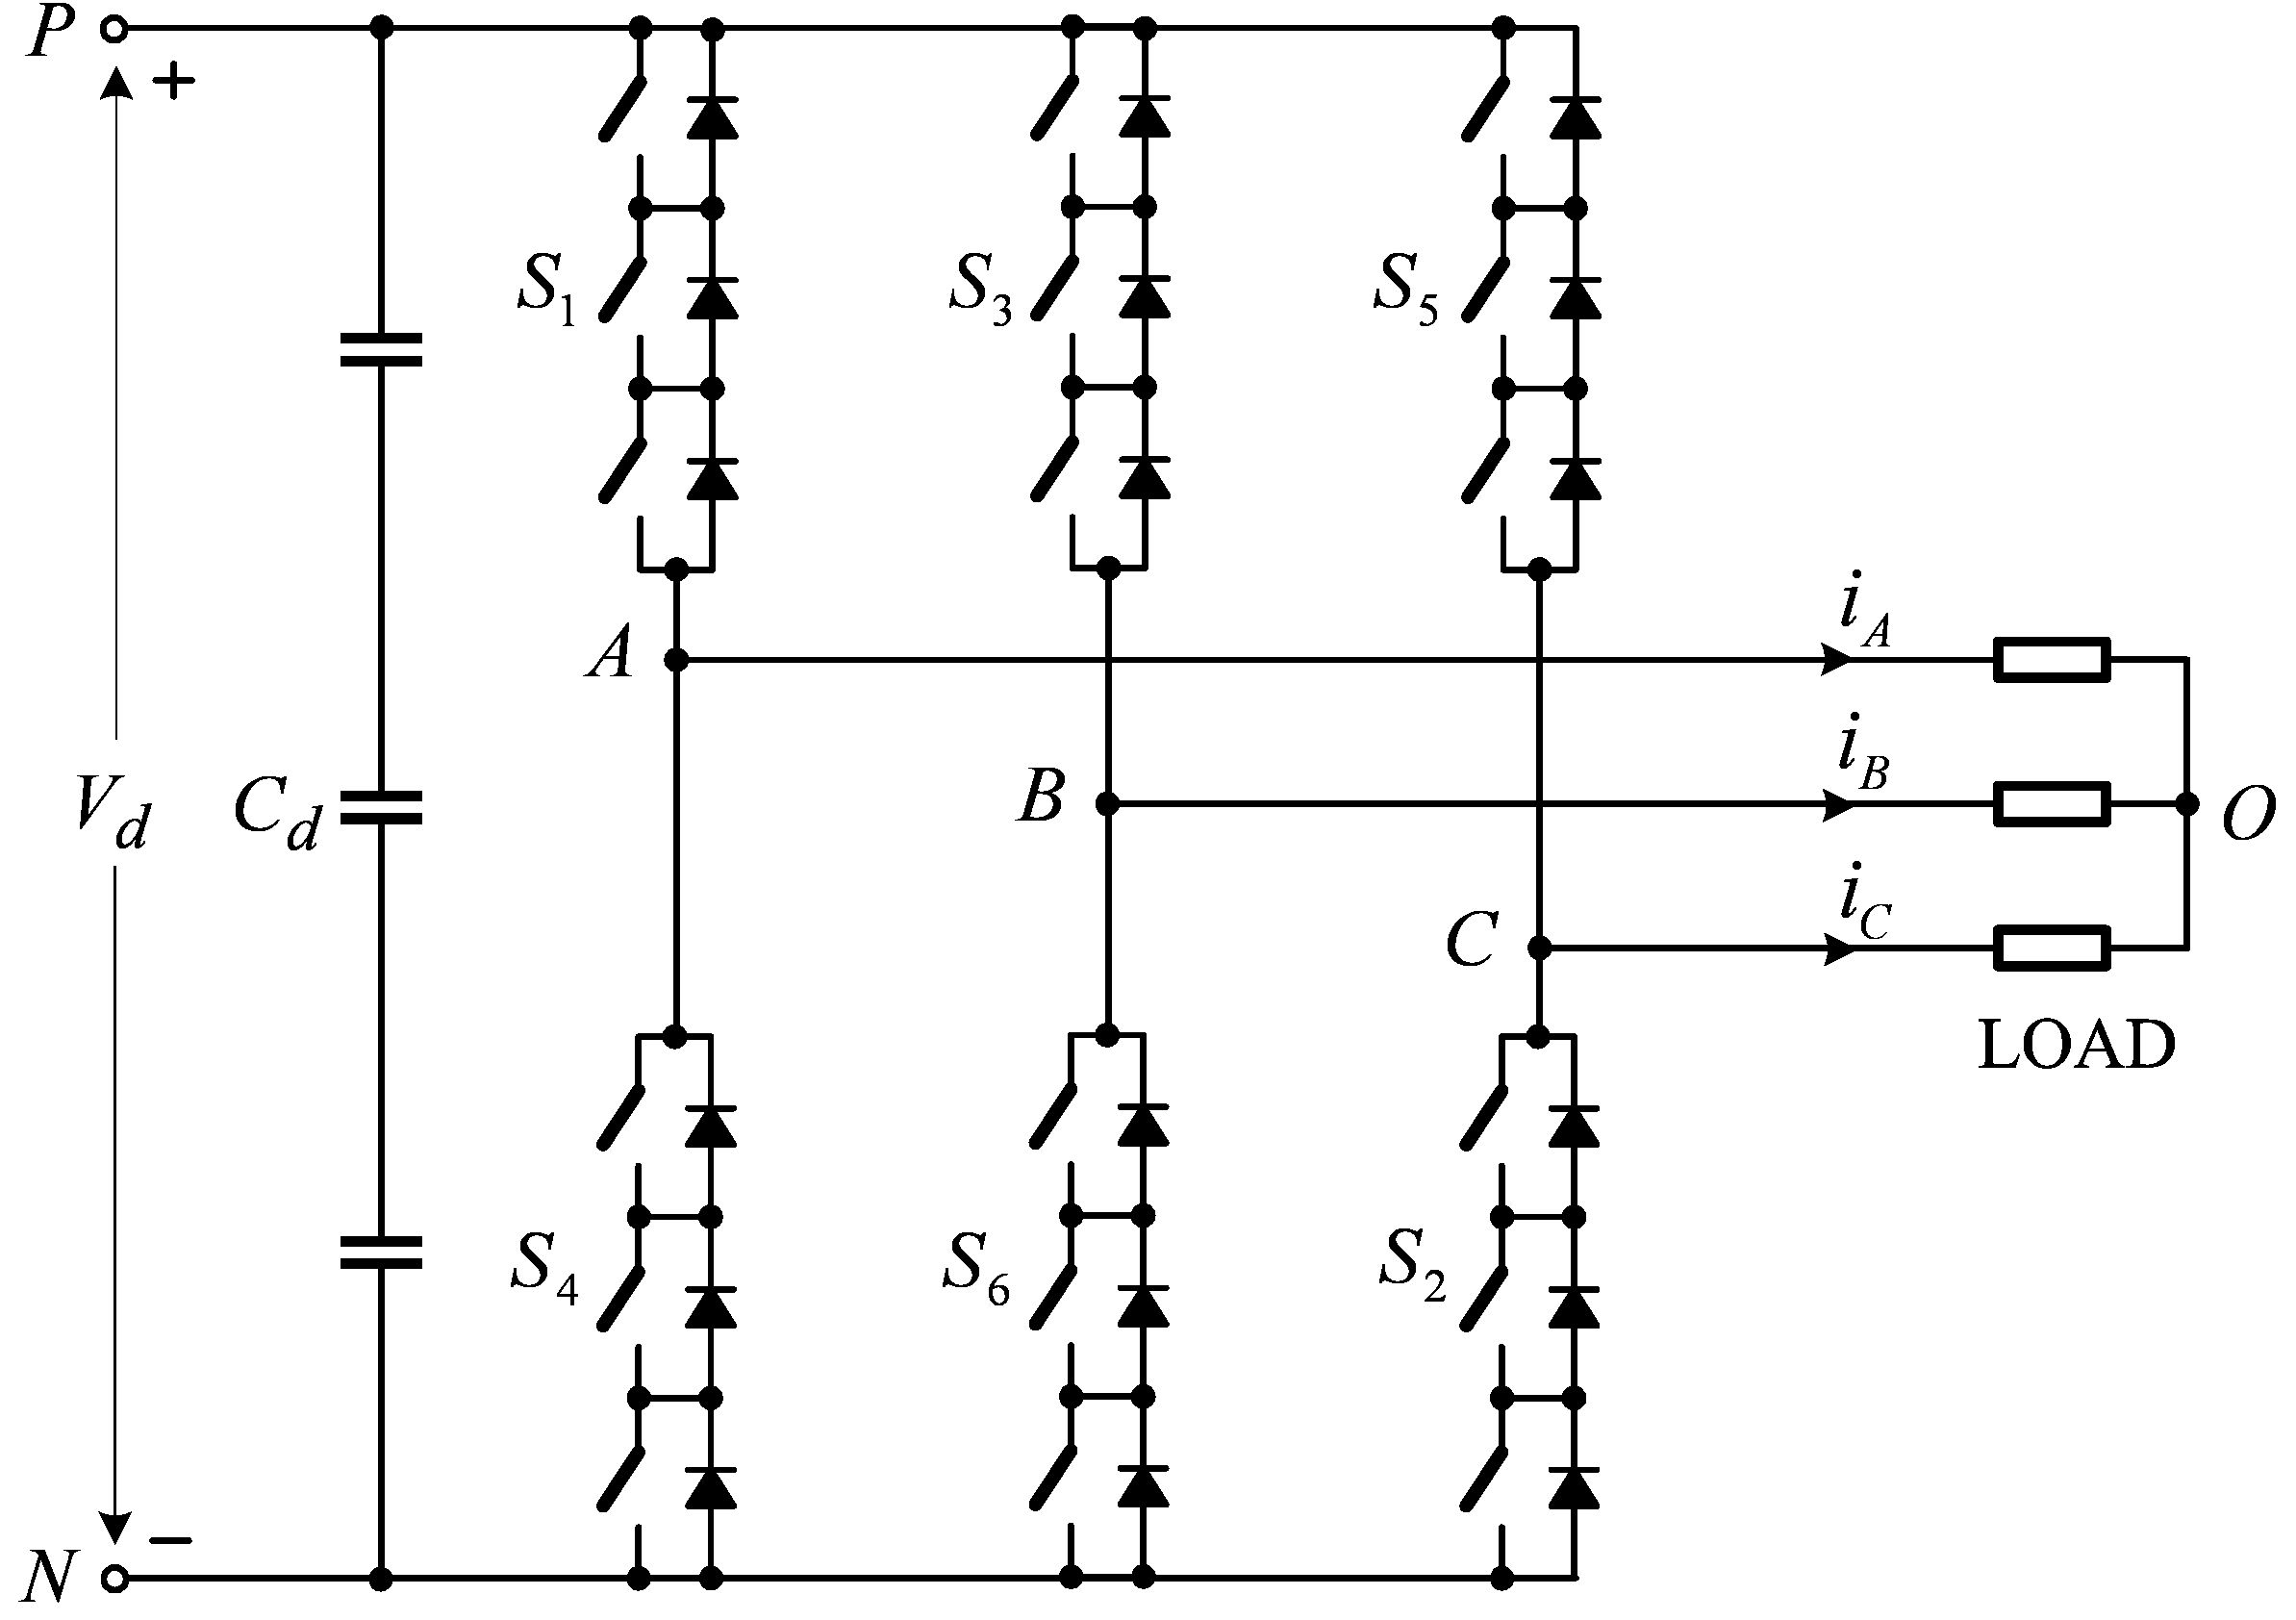
\includegraphics[width=0.8\textwidth]{graficos/img61.jpg}
	\caption{Figura 6.1-1 Inversor de dos niveles simplificado para aplicaciones de alta potencia.}
\end{figure}
\FloatBarrier

\begin{figure}[h]
	\centering
	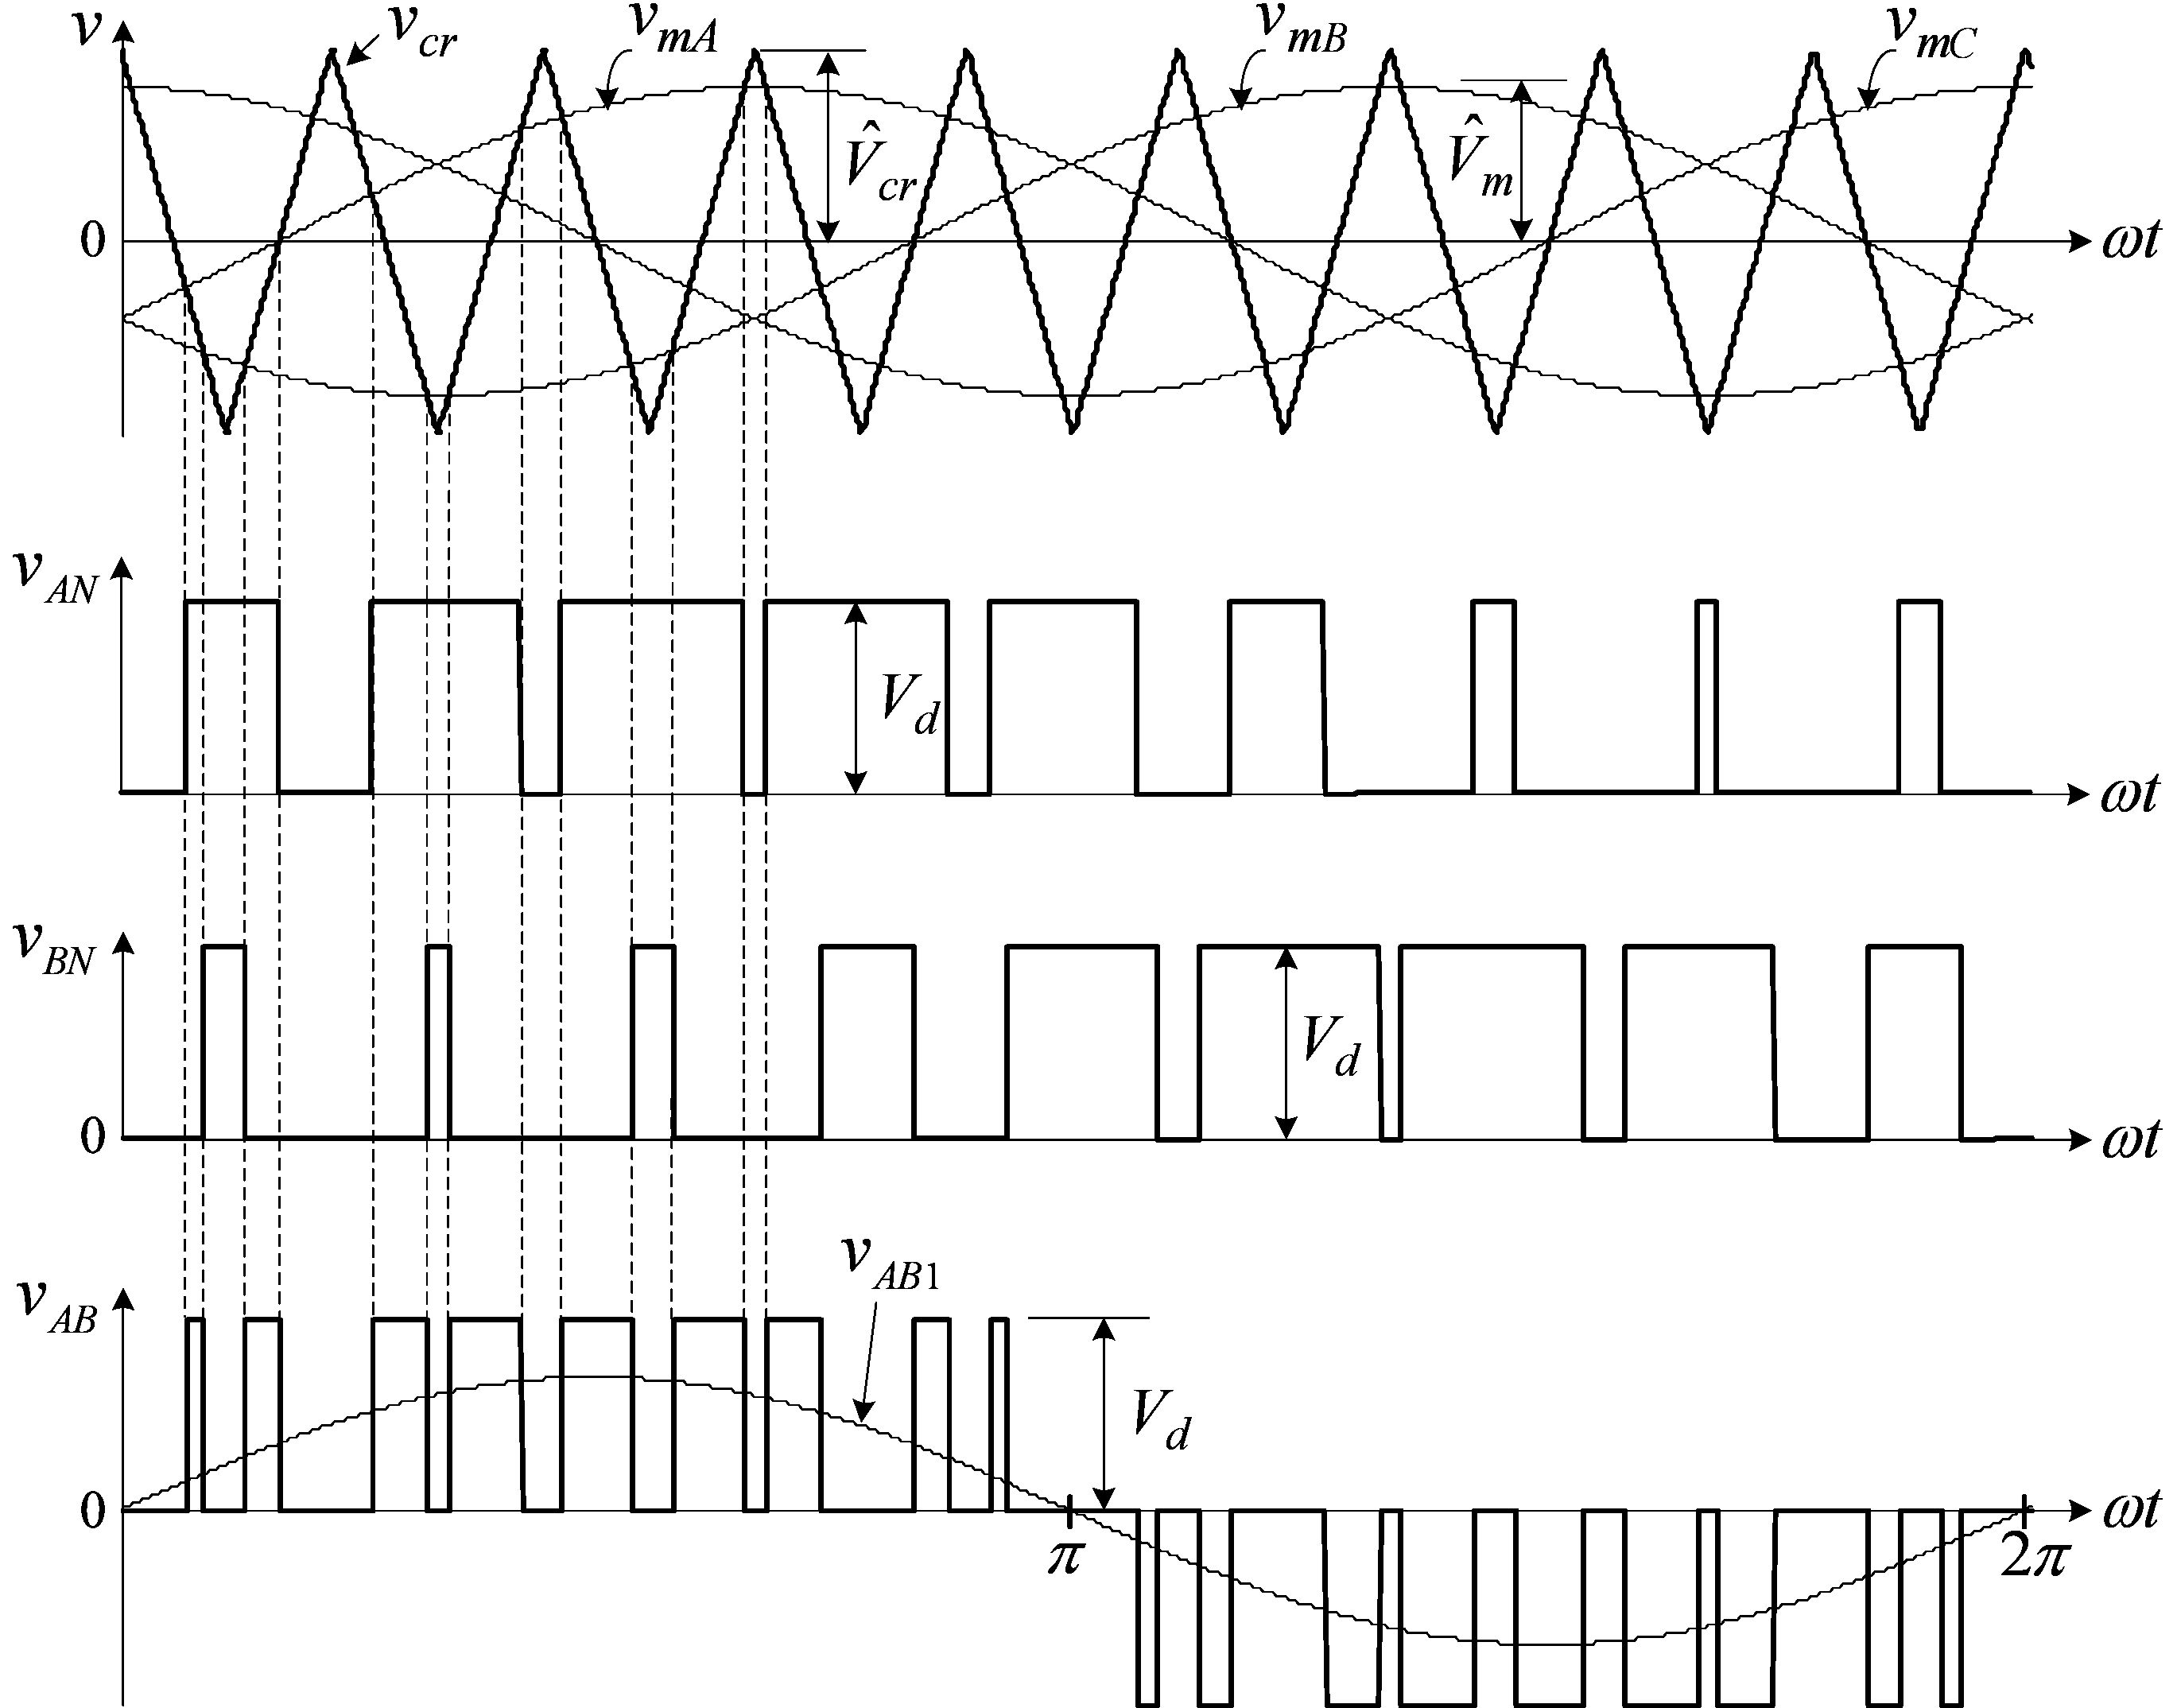
\includegraphics[width=0.8\textwidth]{graficos/img62.jpg}
	\caption{Figura 6.2-1 Modulación por ancho de pulso sinusoidal (SPWM).}
\end{figure}
\FloatBarrier

donde $V_m$ y $V_{cr}$ son los valores pico de las ondas moduladora y portadora, respectivamente. El índice de modulación de amplitud $m_a$ generalmente se ajusta variando $V_m$ mientras se mantiene fijo $V_{cr}$. El \textbf{índice de modulación de frecuencia} se define por
\[
	m_f = \frac{f_{cr}}{f_m}
\]
donde $f_m$ y $f_{cr}$ son las frecuencias de las ondas moduladora y portadora, respectivamente.

El funcionamiento de los interruptores $S_1$ a $S_6$ se determina comparando las ondas moduladoras con la onda portadora. Cuando $V_{m_a} > V_{cr}$, el interruptor superior $S_1$ en la rama A del inversor se enciende. El interruptor inferior $S_4$ opera de manera complementaria y, por lo tanto, se apaga. El \textit{voltaje terminal del inversor} $V_{AN}$, que es el voltaje en el terminal de fase A respecto al bus DC negativo $N$, es igual al voltaje DC $V_d$. Cuando $V_{m_a} < V_{cr}$, $S_1$ está encendido y $S_4$ está apagado, lo que lleva a $V_{AN} = 0$, como se muestra en la Figura 6.2-1. Dado que la forma de onda de $V_{AN}$ tiene solo dos niveles, $V_d$ y 0, el inversor se conoce como \textit{inversor de dos niveles}. Cabe señalar que para evitar posibles cortocircuitos durante las transiciones de conmutación de los dispositivos superiores e inferiores en una rama del inversor, se debe implementar un \textit{tiempo de bloqueo}, durante el cual ambos interruptores están apagados.

El voltaje línea a línea del inversor $V_{AB}$ puede determinarse por $V_{AB} = V_{AN} - V_{BN}$. La forma de onda de su componente de frecuencia fundamental $V_{AB1}$ también se da en la figura. La magnitud y frecuencia de $V_{AB1}$ pueden controlarse de manera independiente mediante $m_a$ y $f_m$, respectivamente.

La \textbf{frecuencia de conmutación} de los interruptores activos en el inversor de dos niveles se puede encontrar a partir de $f_{sw} = f_{cr} - f_m \times m_f$. Por ejemplo, $V_{AN}$ en la Figura 6.2-1 contiene nueve pulsos por ciclo de la frecuencia fundamental. Cada pulso se produce al encender y apagar una vez $S_1$. Con una frecuencia fundamental de 60 Hz, la frecuencia de conmutación resultante para $S_1$ es $f_{sw} = 60 \times 9 = 540$ Hz, que también es la frecuencia de la portadora $f_{cr}$. Vale la pena notar que la frecuencia de conmutación de los dispositivos no siempre puede ser igual a la frecuencia de la portadora en inversores multinivel. Este tema se abordará en los capítulos posteriores.

Cuando la onda portadora está sincronizada con la onda moduladora ($m_f$ es un entero), el esquema de modulación se conoce como \textbf{PWM sincrónico}, en contraste con el \textbf{PWM asincrónico} cuya frecuencia de portadora $f_{cr}$ generalmente es fija e independiente de $f_m$. El PWM asincrónico presenta una frecuencia de conmutación fija y una fácil implementación con circuitos analógicos. Sin embargo, puede generar armónicos no característicos, cuya frecuencia no es múltiplo de la frecuencia fundamental. El esquema PWM sincrónico es más adecuado para la implementación con un procesador digital.

\subsubsection{Contenido Armónico}
La Figura 6.2-2 muestra un conjunto de formas de onda simuladas para el inversor de dos niveles, donde $V_{AB}$ es el voltaje línea a línea del inversor, $V_{A0}$ es el voltaje de fase de la carga e $i_4$ es la corriente de la carga. El inversor opera bajo la condición de $m_a = 0.8$, $m_f = 15$, $f_m = 60$ Hz, y $f_{sw} = 900$ Hz con una carga inductiva trifásica nominal. El factor de potencia de la carga es 0.9 por fase. Podemos observar lo siguiente:

\begin{itemize}
	\item Todos los armónicos en $V_{AB}$ con orden inferior a $(m_f - 2)$ son eliminados.
	\item Los armónicos están centrados alrededor de $m_f$ y sus múltiplos como $2m_f$ y $3m_f$.
\end{itemize}

Las declaraciones anteriores son válidas para $m_f \geq 9$ siempre que $m_f$ sea un múltiplo de 3 \cite{ref1}. La forma de onda de la corriente de carga $i_4$ es cercana a sinusoidal con una distorsión armónica total (THD) de 7.73\%. La baja cantidad de distorsión armónica se debe a la eliminación de armónicos de orden bajo por el esquema de modulación y al efecto de filtrado de la inductancia de la carga.

\begin{figure}[h]
	\centering
	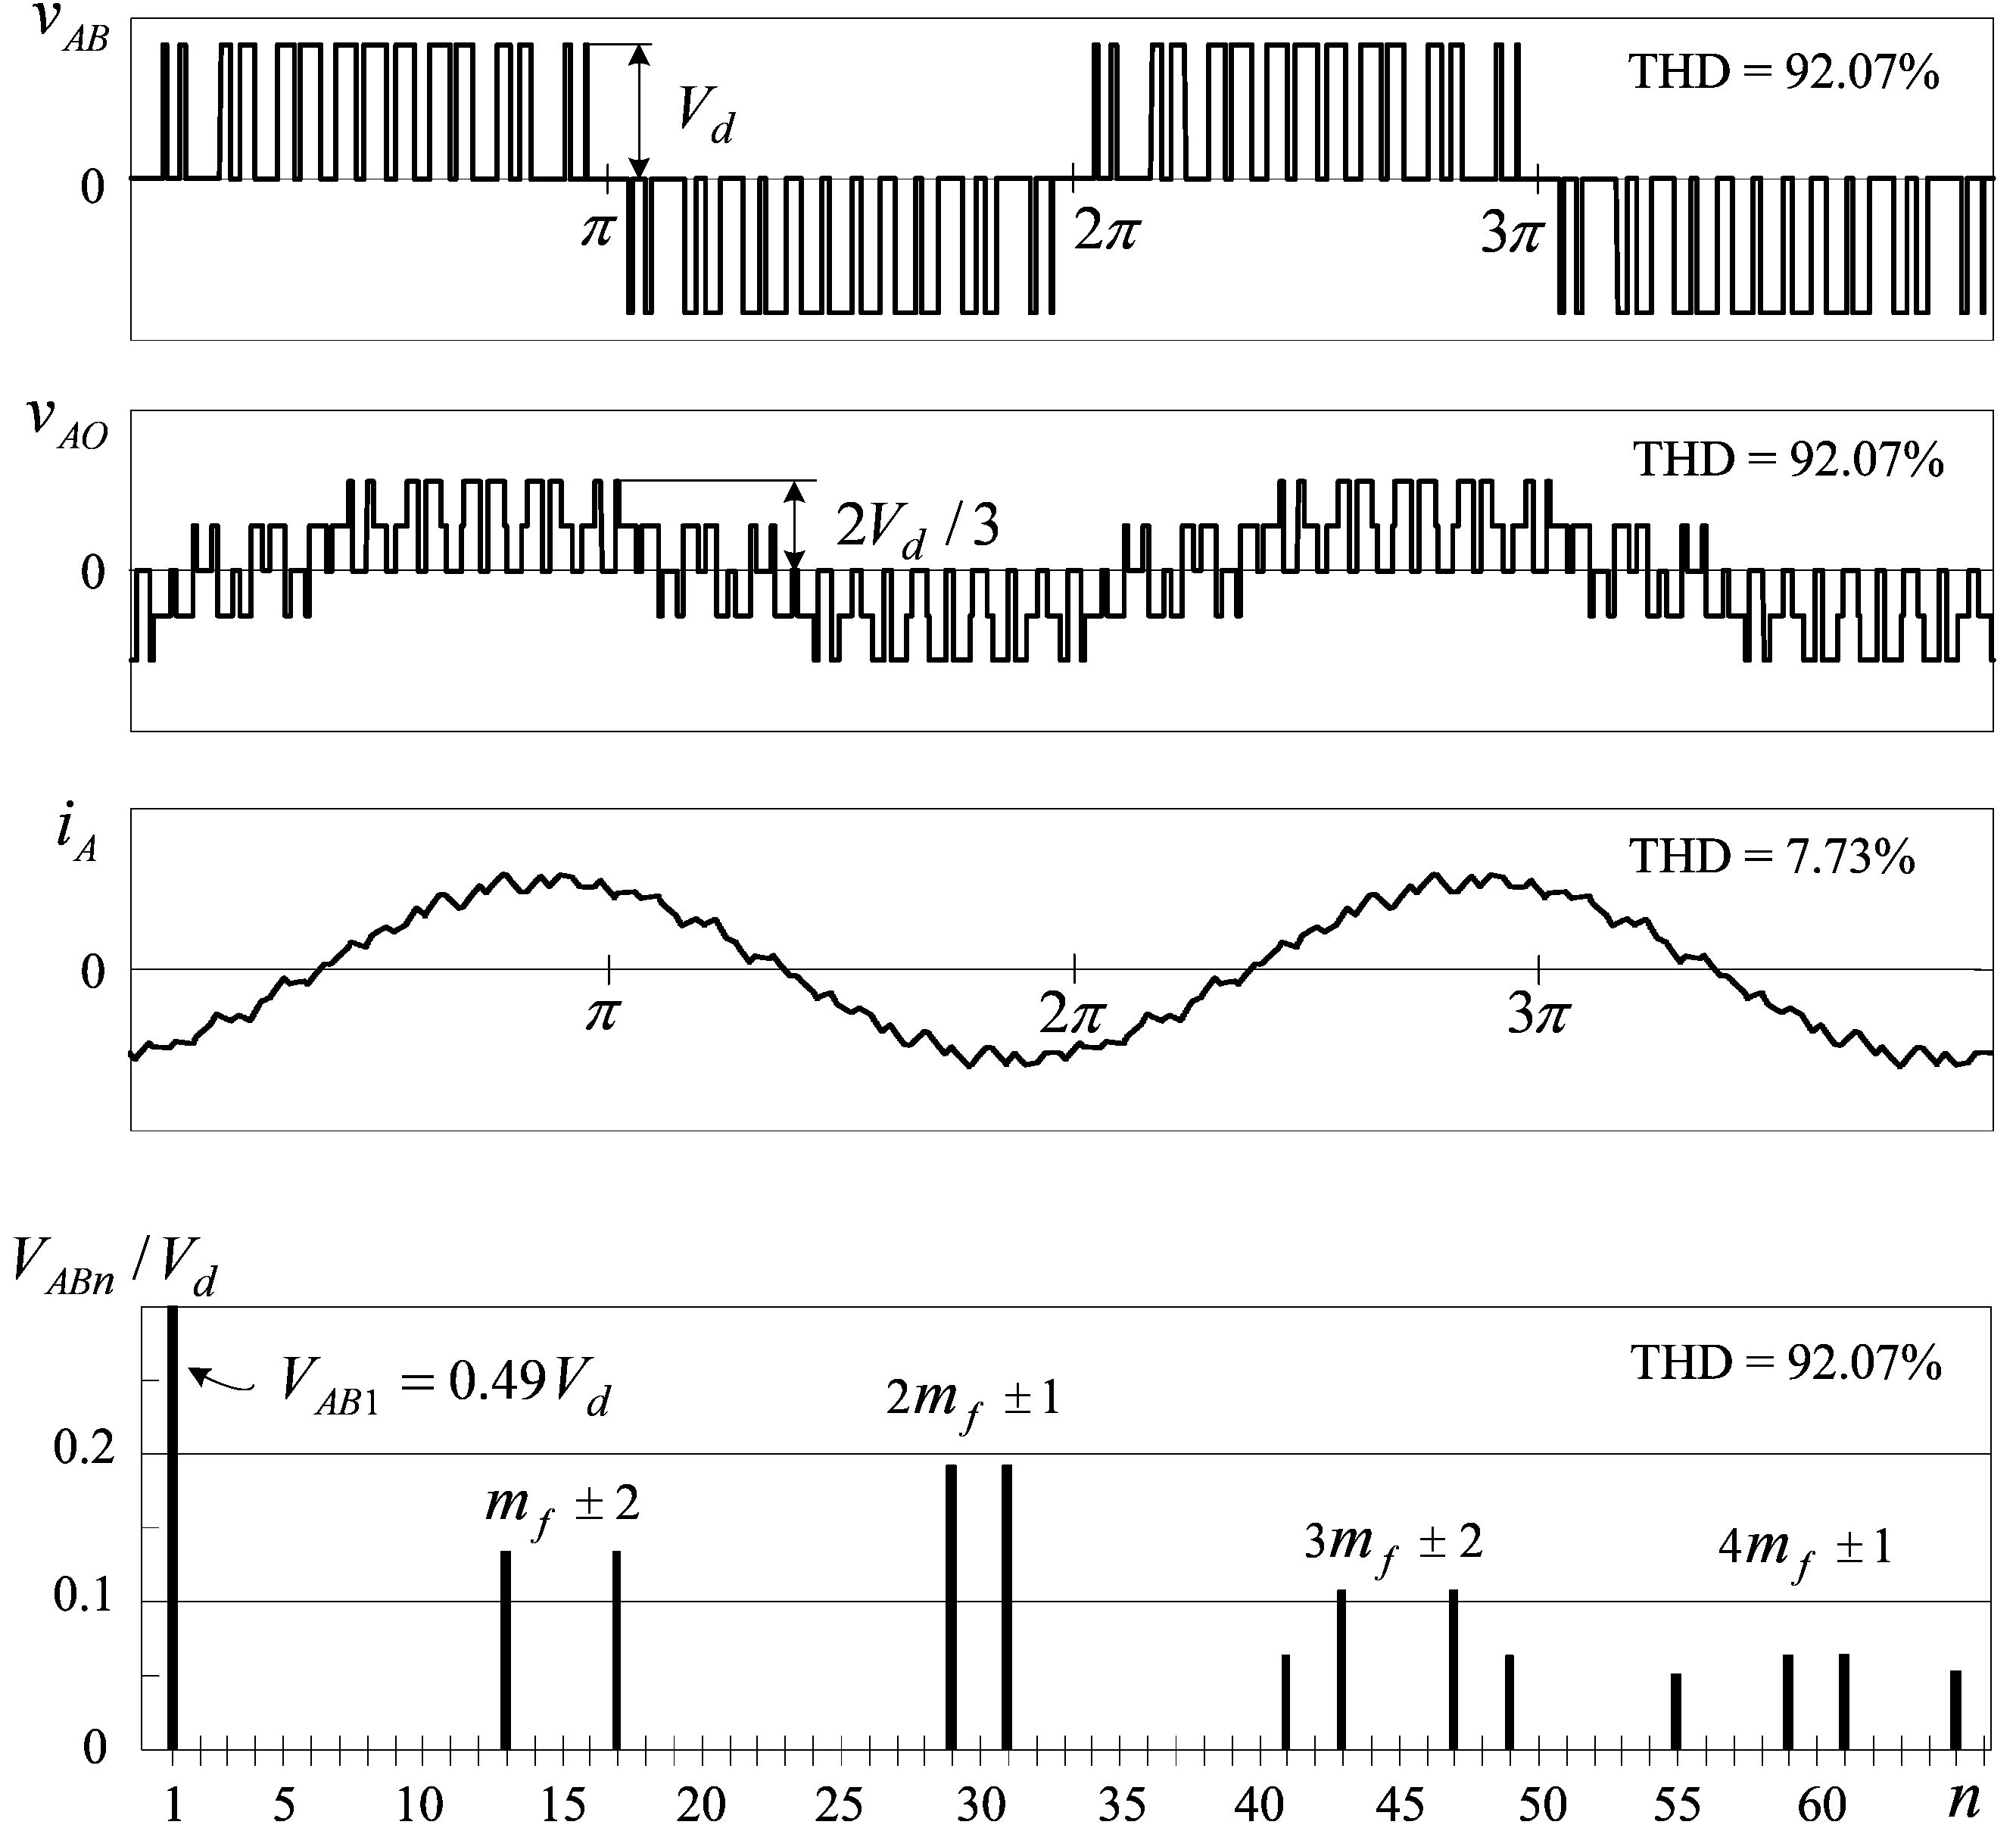
\includegraphics[width=0.9\textwidth]{graficos/img71.jpg}
	\caption{Figura 6.2-3 Formas de onda simuladas para el inversor de dos niveles operando a $m_a = 0.8$, $m_f = 15$, $f_m = 60$ Hz, y $f_{sw} = 900$ Hz.}
\end{figure}
\FloatBarrier

\begin{figure}[h]
	\centering
	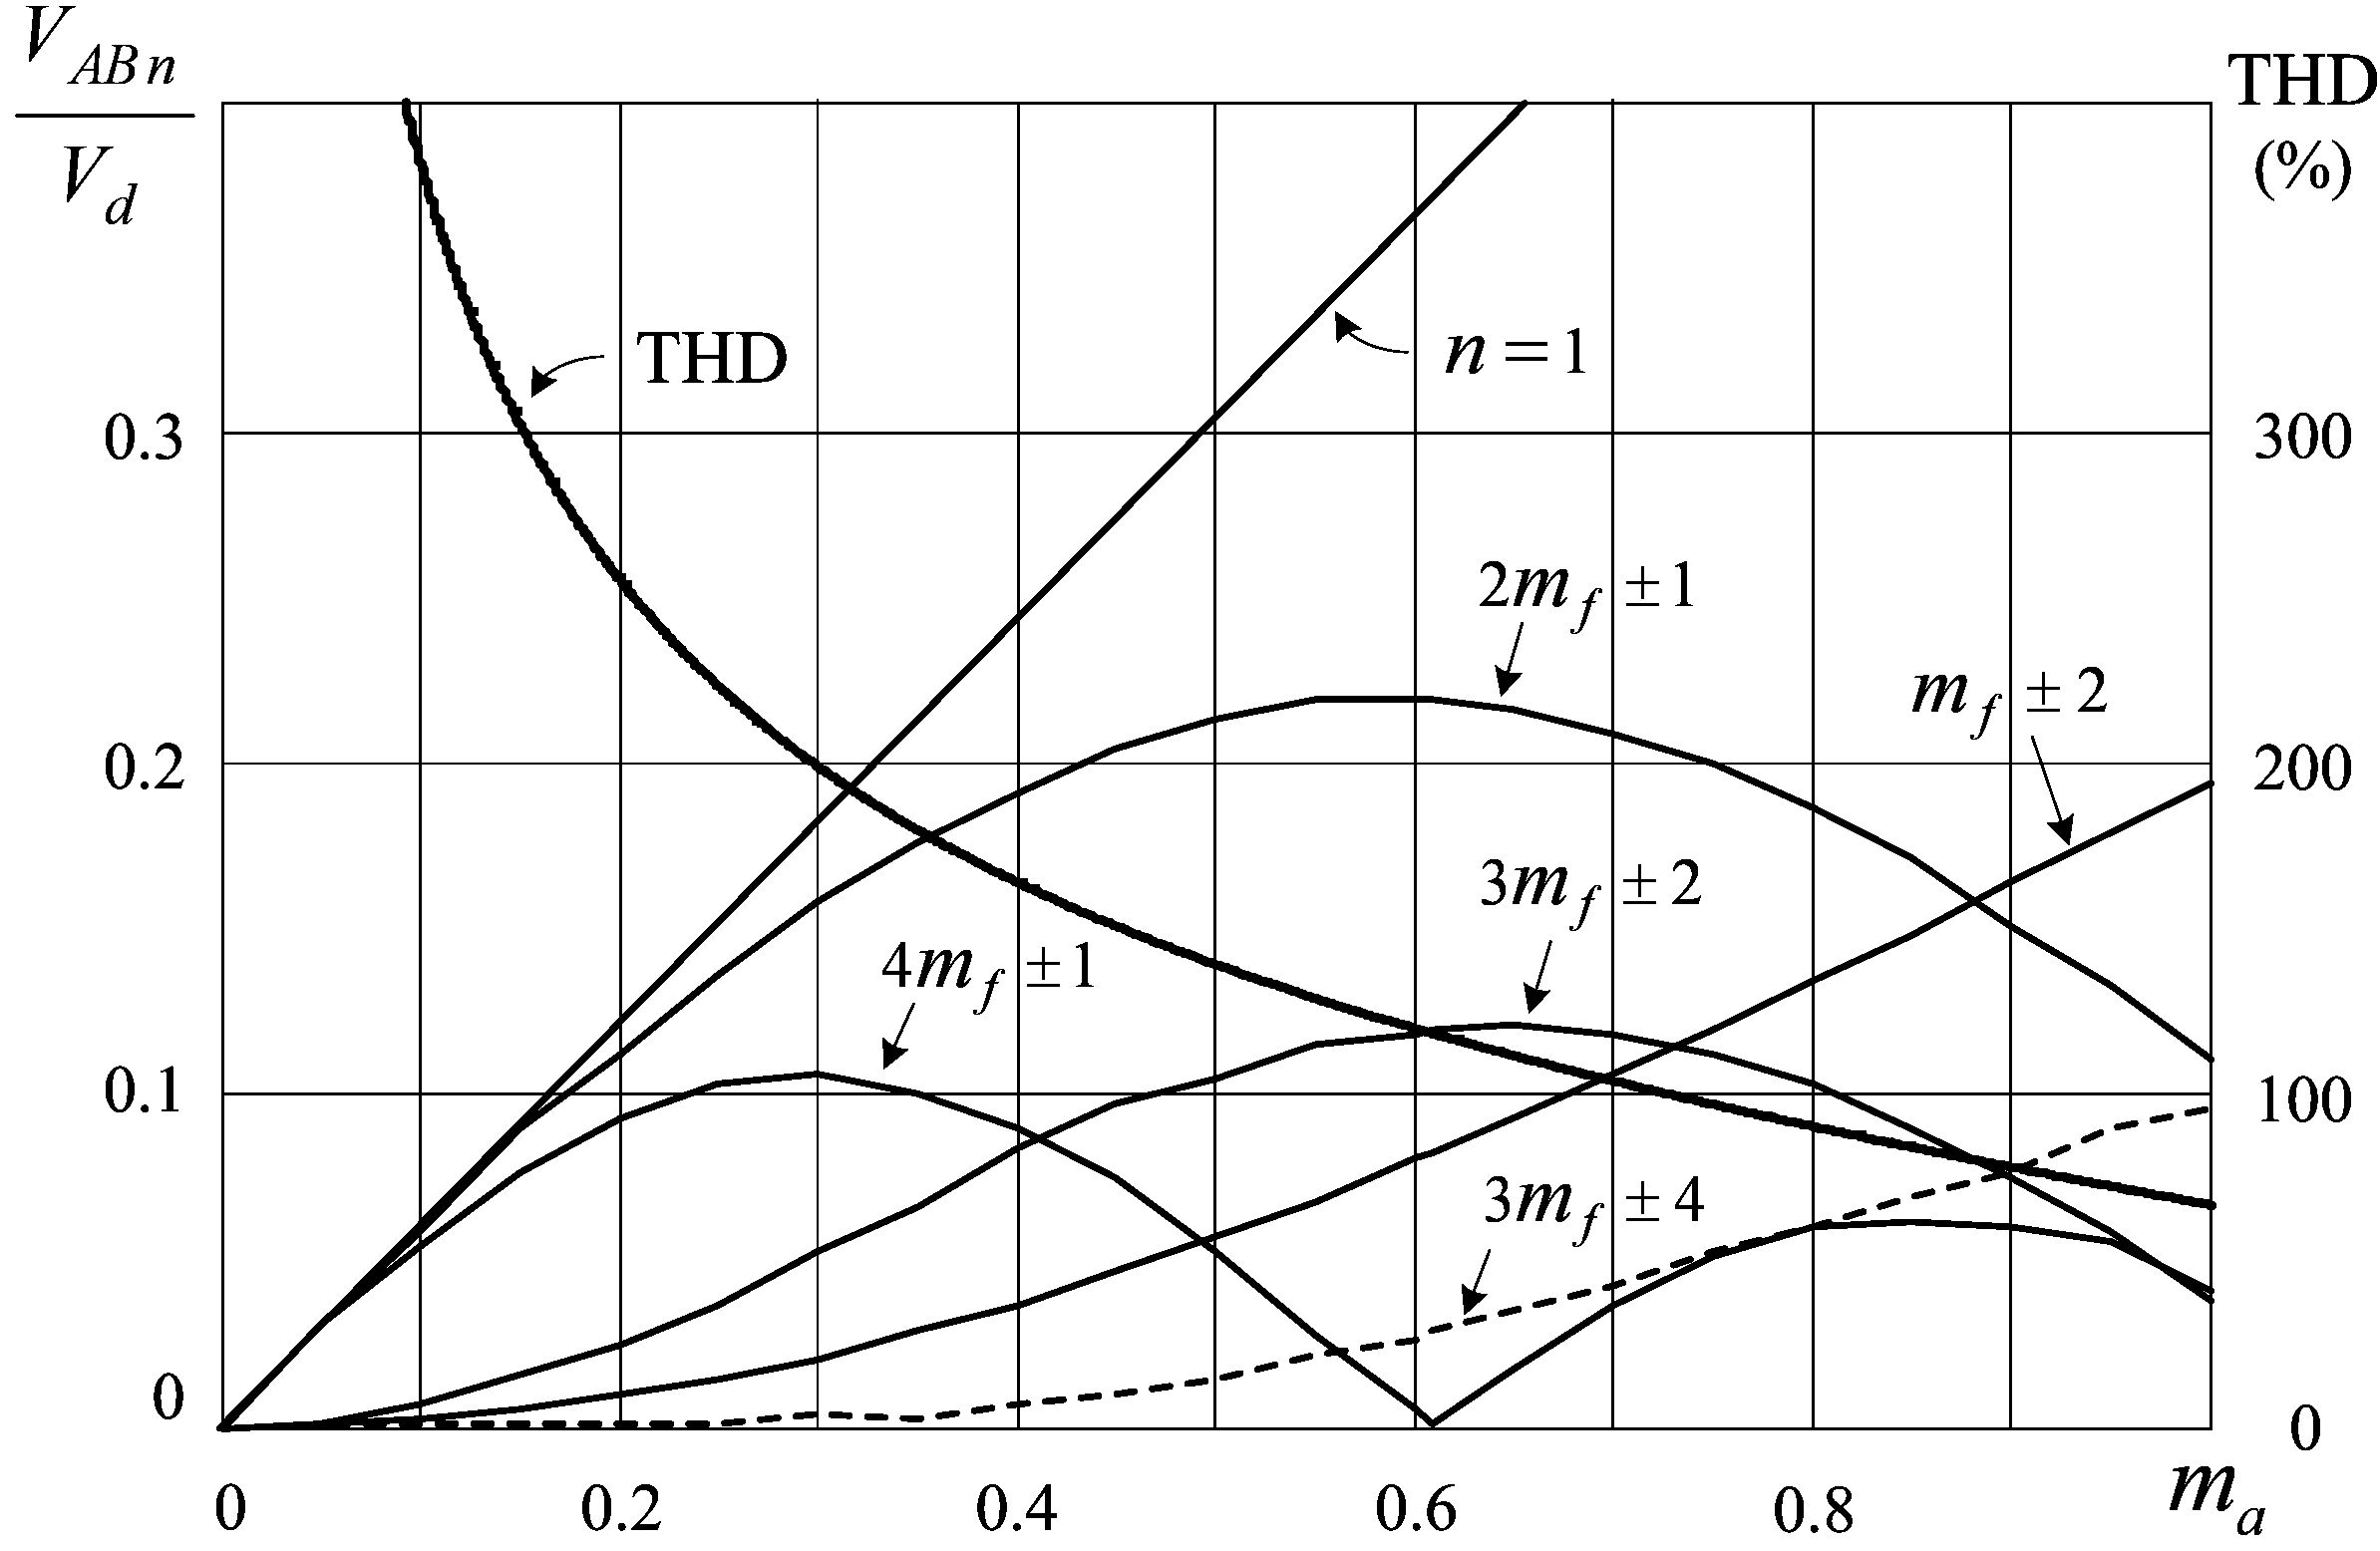
\includegraphics[width=0.8\textwidth]{graficos/img80.jpg}
	\caption{Figura 6.2-3 Contenido armónico de $V_{AB}$ en la Figura 6.2-2.}
\end{figure}
\FloatBarrier

\subsection{Sobre-Modulación}
La sobre-modulación ocurre cuando el índice de modulación de amplitud $m_a$ es mayor que uno. La Figura 6.2-4 muestra tal caso con $m_a = 2$. La sobre-modulación causa una reducción en el número de pulsos en la forma de onda del voltaje línea a línea, lo que lleva a la aparición de armónicos de orden bajo como el 5º y 11º. Sin embargo, el voltaje fundamental $V_{AB1}$ se incrementa a 0.744$V_d$, lo que representa un aumento del 22\% en comparación con 0.612$V_d$ a $m_a = 1$. Con $m_a$ incrementado aún más a 3.24, $V_{AB}$ se convierte en una onda cuadrada, cuyo voltaje fundamental es $V_{AB1} = 0.78V_d$, que es el valor máximo posible producido por el VSI de dos niveles. La sobre-modulación rara vez se usa en la práctica debido a las dificultades para filtrar los armónicos de orden bajo y la relación no lineal entre $V_{AB1}$ y $m_a$.

\subsubsection{PWM con Inyección de Armónico de Tercer Orden}
El voltaje fundamental del inversor $V_{AB1}$ también puede incrementarse añadiendo un componente armónico de tercer orden a la onda moduladora sinusoidal trifásica sin causar sobre-modulación. Esta técnica de modulación se conoce como \textit{PWM con inyección de armónico de tercer orden}.

La Figura 6.2-5 ilustra el principio de este esquema de PWM, donde la onda moduladora $v_{m4}$ está compuesta por un componente fundamental $v_{m1}$ y un componente de tercer orden $v_{m3}$, haciendo que $v_{m4}$ se aplane un poco en la parte superior. Como resultado, el componente fundamental pico $v_{m1}$ puede ser mayor que la onda portadora triangular pico $v_{cr}$, lo que potencia el voltaje fundamental $V_{AB1}$. Al mismo tiempo, la onda moduladora pico $v_{m4}$ puede mantenerse por debajo de $v_{cr}$, evitando los problemas causados por la sobre-modulación. La cantidad máxima de $V_{AB1}$ que puede incrementarse mediante este esquema es del 15.5\% \cite{ref2, ref3}.

\begin{figure}[h]
	\centering
	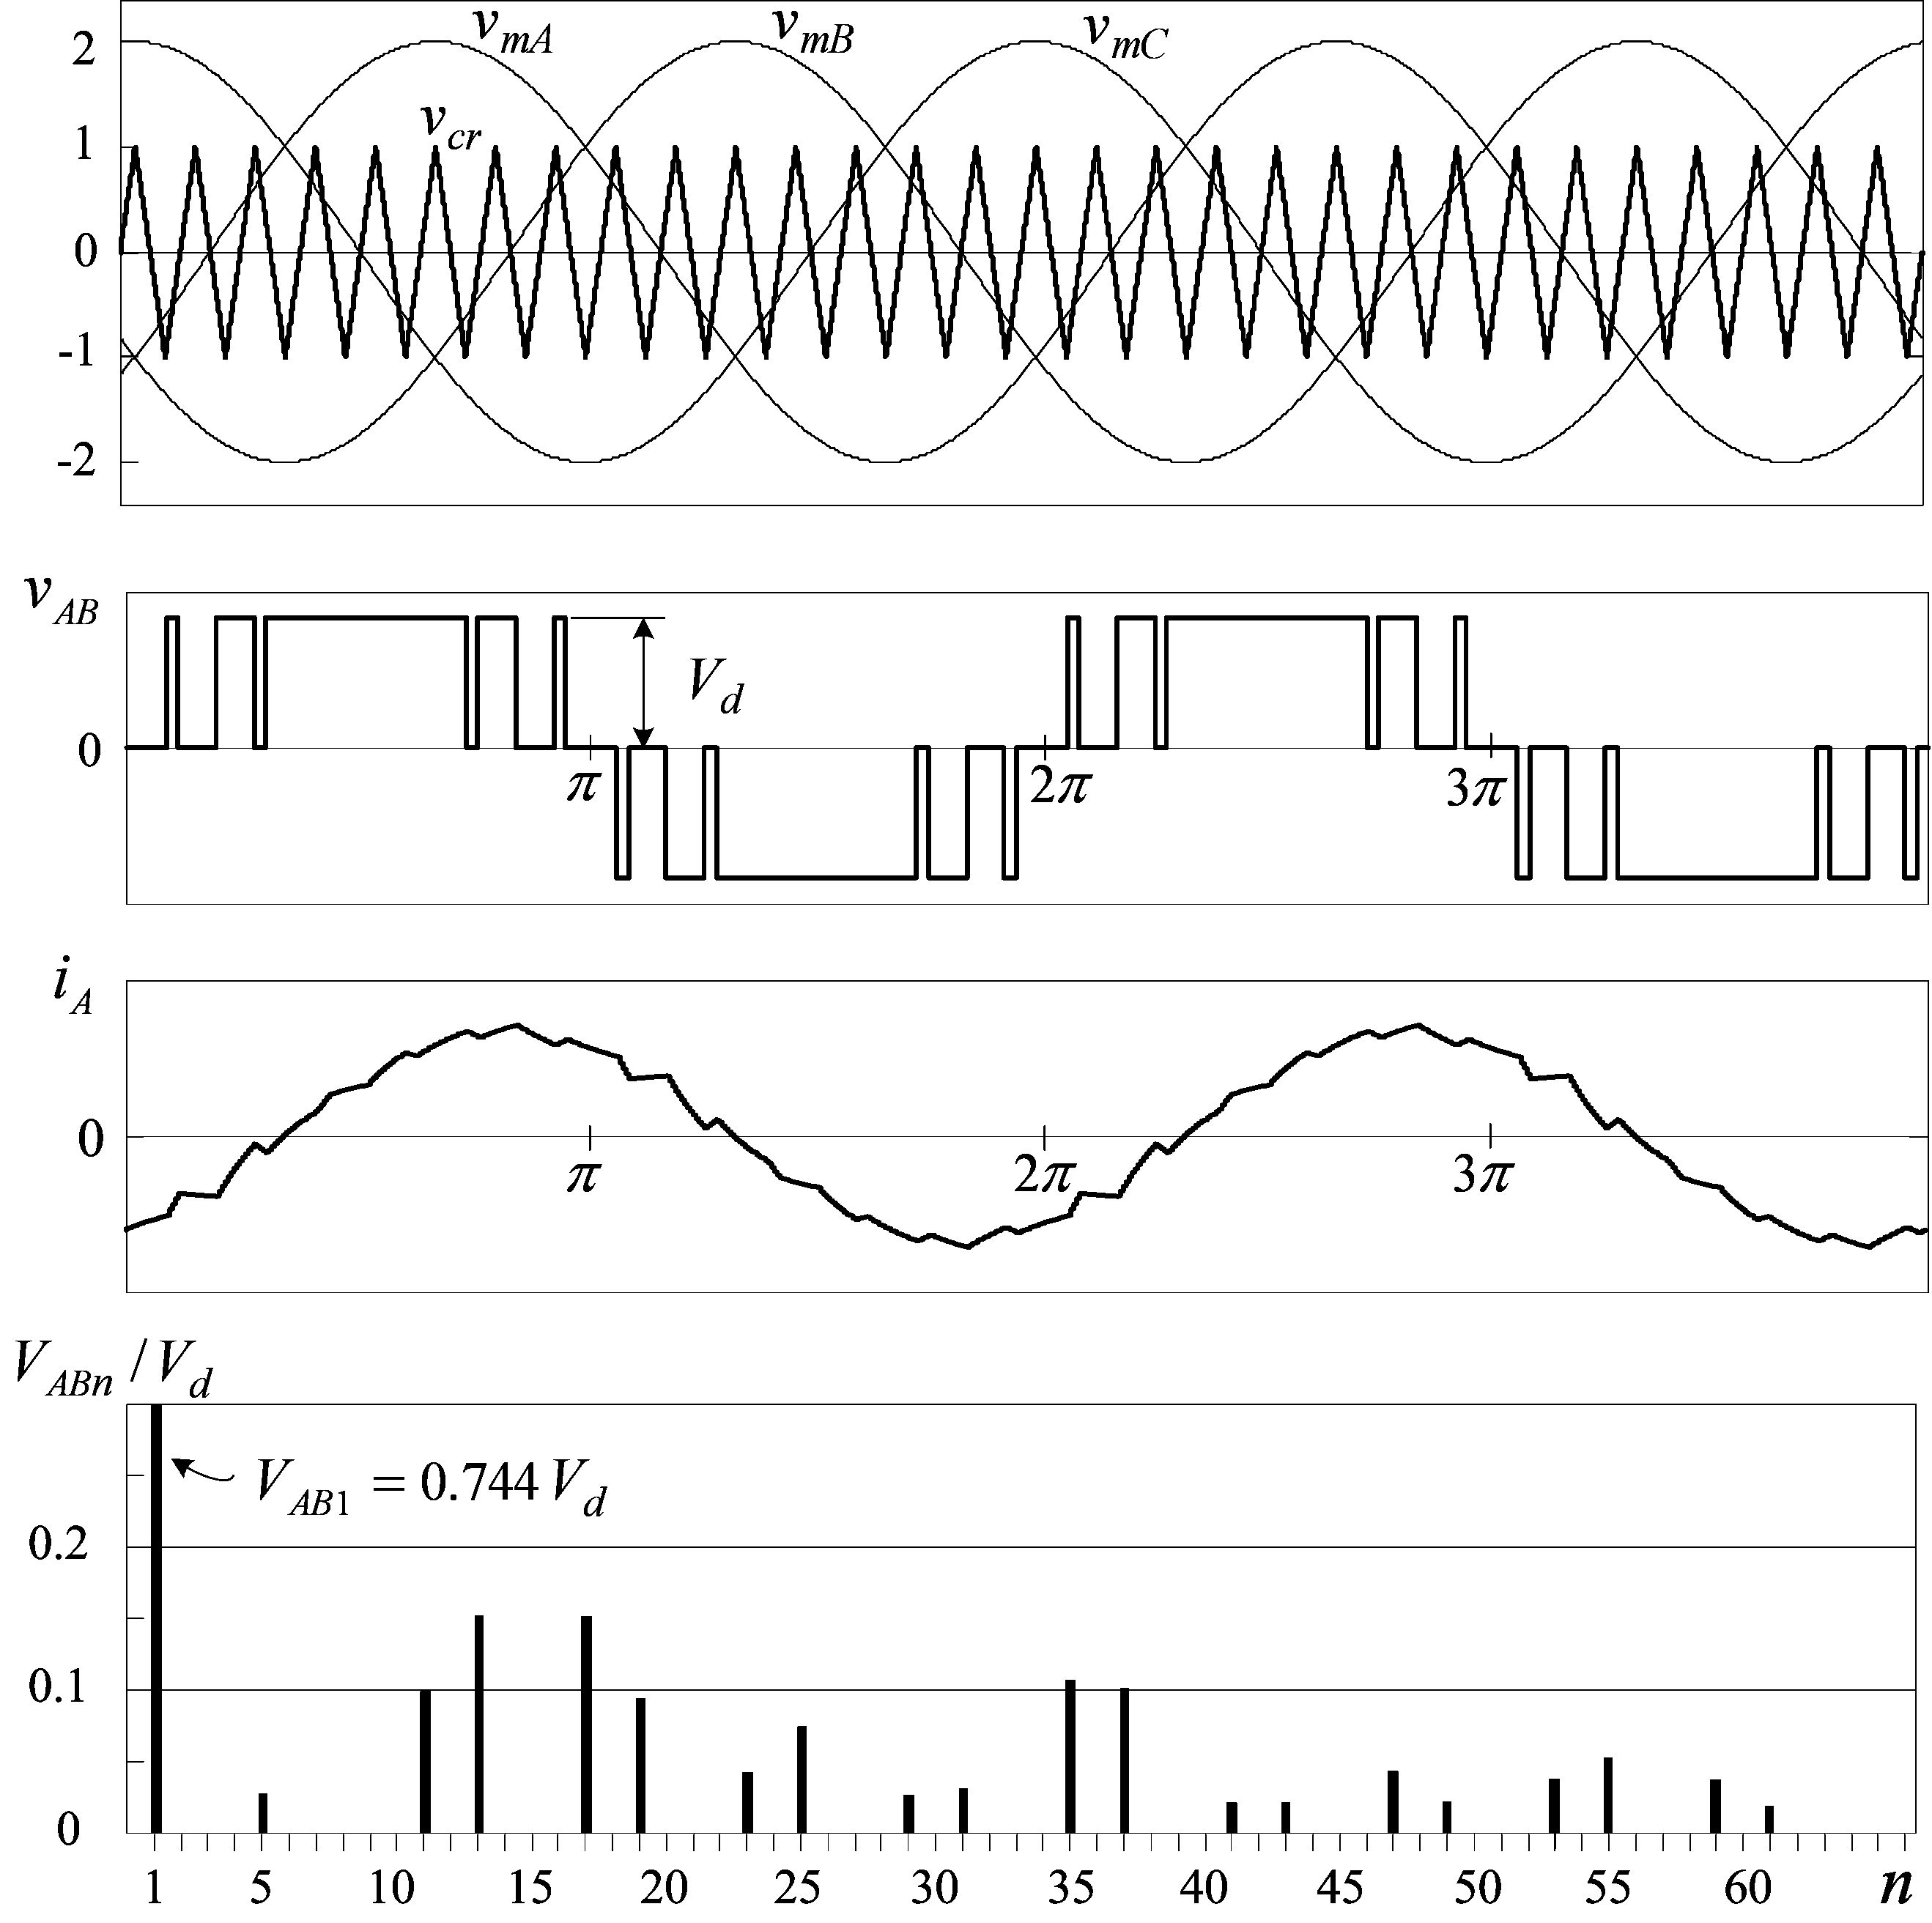
\includegraphics[width=0.8\textwidth]{graficos/img85.jpg}
	\caption{Figura 6.2-4 Sobre-modulación ($m_a = 2.0$, $m_f = 15$, y $f_m = 60$ Hz).}
\end{figure}
\FloatBarrier

\begin{figure}[h]
	\centering
	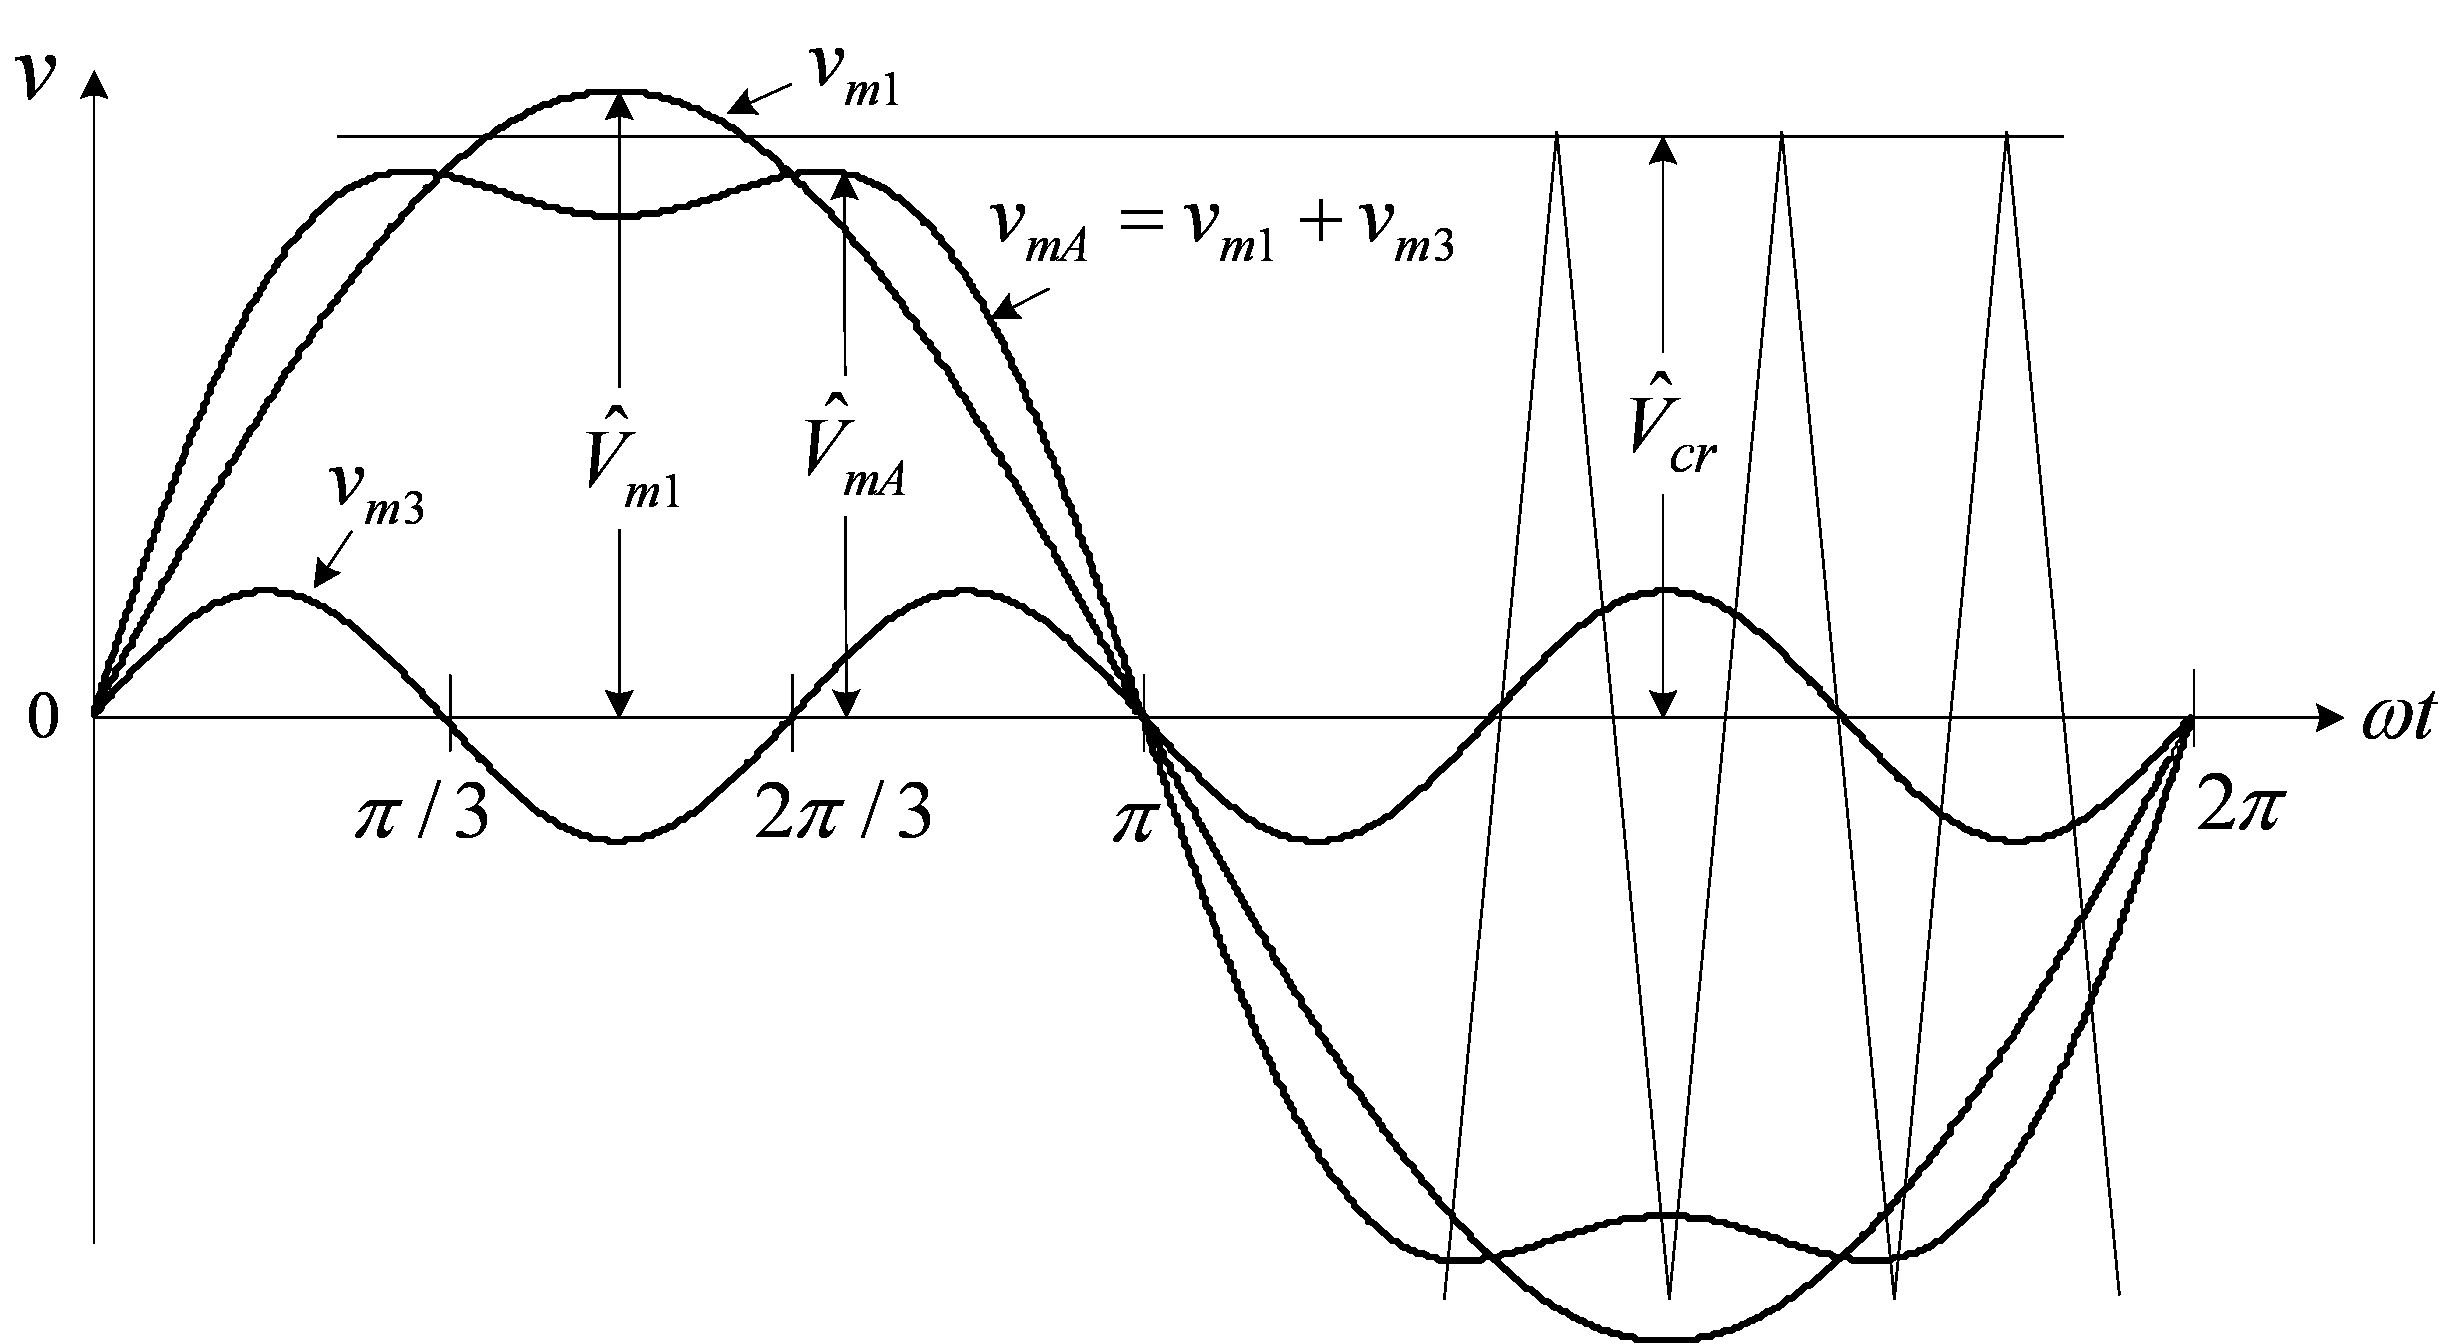
\includegraphics[width=0.8\textwidth]{graficos/img86.jpg}
	\caption{Figura 6.2-5 Onda moduladora $v_{m4}$ con inyección de tercer orden.}
\end{figure}
\FloatBarrier

El componente armónico de tercer orden inyectado $v_{m3}$ no incrementará la distorsión armónica para $V_{AB}$. Aunque aparece en cada uno de los voltajes terminales del inversor $V_{AN}$, $V_{BN}$ y $V_{CN}$, el voltaje armónico de tercer orden no existe en el voltaje línea a línea $V_{AB}$. Esto se debe a que el voltaje línea a línea está dado por $V_{AB} = V_{AN} - V_{BN}$, donde los armónicos de tercer orden en $V_{AN}$ y $V_{BN}$ son de secuencia cero con la misma magnitud y desplazamiento de fase, por lo que se cancelan entre sí.

\section{Modulación Vectorial de Espacio}
La modulación vectorial de espacio (SVM) es una de las técnicas de modulación preferidas en tiempo real y es ampliamente utilizada para el control digital de inversores de fuente de voltaje \cite{ref3, ref4}. Esta sección presenta el principio e implementación de la modulación vectorial de espacio para el inversor de dos niveles.

\subsection{Estados de Conmutación}
El estado de operación de los interruptores en el inversor de dos niveles en la Figura 6.1-1 puede representarse mediante estados de conmutación. Como se indica en la Tabla 6.3-1, el estado de conmutación `P' denota que el interruptor superior en una rama del inversor está encendido y el voltaje terminal del inversor ($V_{AN}$, $V_{BN}$ o $V_{CN}$) es positivo ($+V_d$) mientras que `O' indica que el voltaje terminal del inversor es cero debido a la conducción del interruptor inferior.

\begin{table}[h]
    \centering
    \caption{Tabla 6.3-1 Definición de Estados de Conmutación}
    \begin{tabular}{c c c c c c c c c c}
        \hline
        \textbf{Conmutación} & & \textbf{Rama A} & & & \textbf{Rama B} & & & \textbf{Rama C} & \\
        \hline
        \textbf{Estado} & $S_1$ & $S_4$ & $V_{AN}$ & $S_3$ & $S_6$ & $V_{BN}$ & $S_5$ & $S_2$ & $V_{CN}$ \\
        \hline
        P & Encendido & Apagado & $V_d$ &  Encendido & Apagado & $V_d$ & Encendido & Apagado & $V_d$ \\
        O & Apagado & Encendido & 0 & Apagado & Encendido & 0 & Apagado & Encendido & 0 \\
        \hline
    \end{tabular}
    \label{tabla:estados_conmutacion}
\end{table}
\FloatBarrier

Hay ocho combinaciones posibles de estados de conmutación en el inversor de dos niveles como se lista en la Tabla 6.3-2. El estado de conmutación [POO], por ejemplo, corresponde a la conducción de $S_1$, $S_6$ y $S_2$ en las ramas A, B y C del inversor, respectivamente. De los ocho estados de conmutación, [PPP] y [OOO] son estados cero y los otros son estados activos.

\begin{table}[h]
    \centering
    \caption{Tabla 6.3-2 Vectores de Espacio, Estados de Conmutación y Interruptores en Estado Activo}
    \begin{tabular}{c c c c c}
    \hline
    & & \textbf{Estado de Conmutación} & & \textbf{Vector} \\
        \textbf{Vector de Espacio}  & & \textbf{(Tres Fases)} & \textbf{Interruptor en Estado Activo} & \textbf{Definición} \\
    \hline
    Vector Cero & $\mathbf{V}_7$ & [PPP] & $S_1, S_3, S_5$ & $\mathbf{V}_0 = 0$ \\
                & $\mathbf{V}_0$ & [OOO] & $S_4, S_6, S_2$ & $\mathbf{V}_0 = 0$ \\ [1em]
    Vector Activo & $\mathbf{V}_1$ & [POO] & $S_1, S_6, S_2$ & $\mathbf{V}_1 = \frac{2}{3} V_{dc}e^{j0}$ \\[0.5em]
    & $\mathbf{V}_2$ & [PPO] & $S_1, S_3, S_2$ & $\mathbf{V}_2 = \frac{2}{3} V_{dc}e^{j\frac{\pi}{3}}$ \\[0.5em]
    & $\mathbf{V}_3$ & [OPO] & $S_4, S_3, S_2$ & $\mathbf{V}_3 = \frac{2}{3} V_{dc}e^{j\frac{2\pi}{3}}$ \\[0.5em]
    & $\mathbf{V}_4$ & [OPP] & $S_4, S_3, S_5$ & $\mathbf{V}_4 = \frac{2}{3} V_{dc}e^{j\pi}$ \\[0.5em]
    & $\mathbf{V}_5$ & [OOP] & $S_4, S_6, S_5$ & $\mathbf{V}_5 = \frac{2}{3} V_{dc}e^{j\frac{4\pi}{3}}$ \\[0.5em]
    & $\mathbf{V}_6$ & [POP] & $S_1, S_6, S_5$ & $\mathbf{V}_6 = \frac{2}{3} V_{dc}e^{j\frac{5\pi}{3}}$ \\[0.5em]
    \hline
    \end{tabular}
    \label{tabla:vectores_espacio}
\end{table}
\FloatBarrier
    
\subsection{Vectores de Espacio}
Los estados de conmutación activos y cero pueden representarse mediante vectores de espacio activos y cero, respectivamente. Un diagrama típico de vectores de espacio para el inversor de dos niveles se muestra en la Figura 6.3-1, donde los seis vectores activos $V_1$ a $V_6$ forman un hexágono regular con seis sectores iguales (I a VI). El vector cero $V_0$ se encuentra en el centro del hexágono.

\begin{figure}[h]
    \centering
    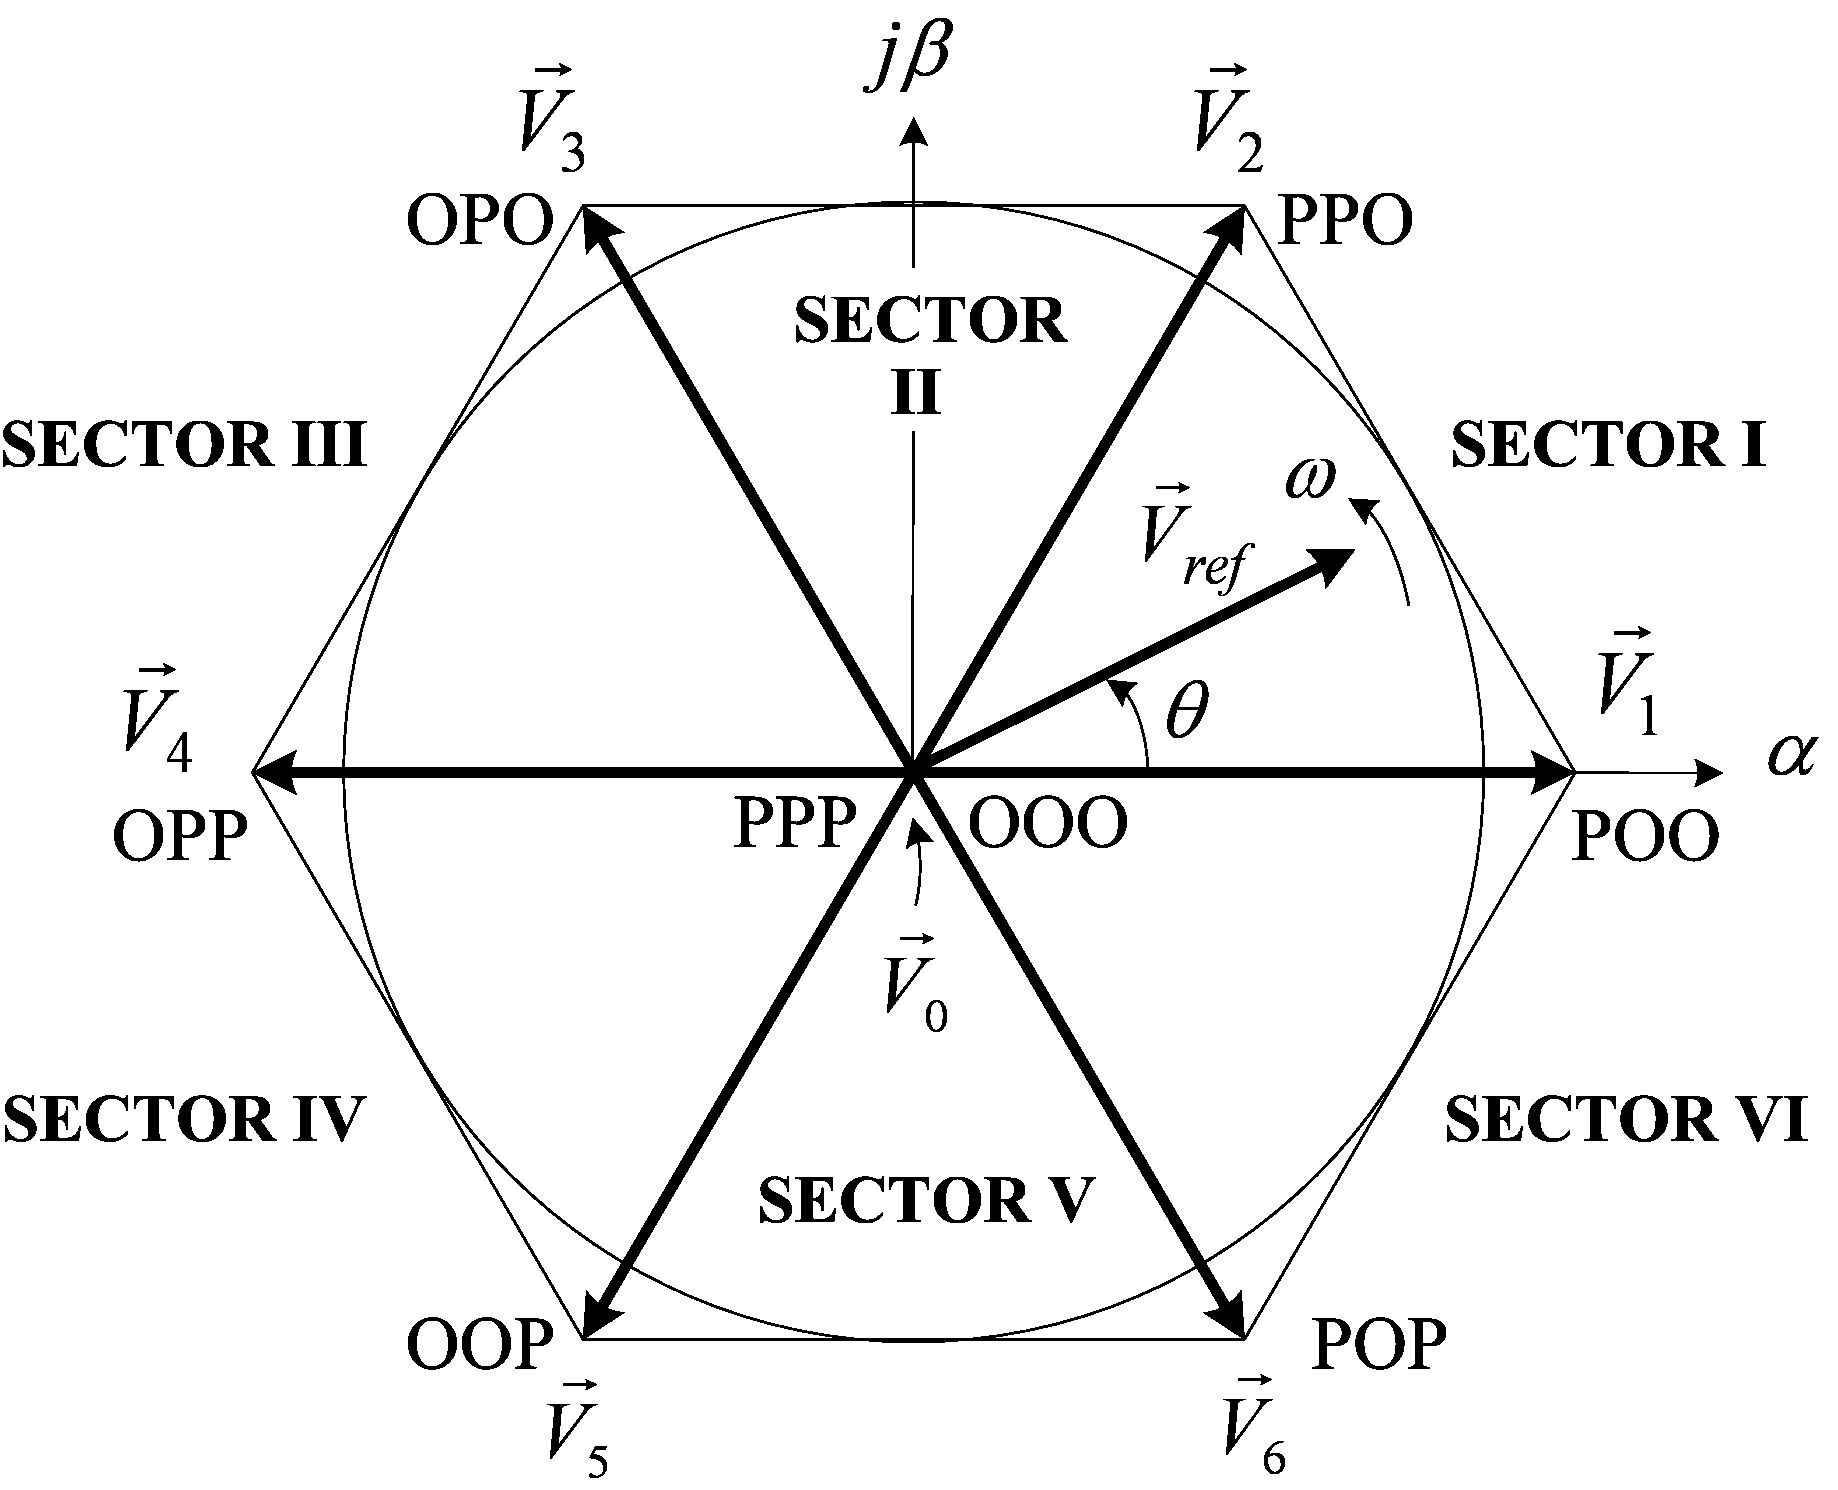
\includegraphics[width=0.8\textwidth]{graficos/img99.jpg}
    \caption{Figura 6.3-1 Diagrama de vectores de espacio para el inversor de dos niveles.}
    \label{fig:diagrama_vectores_espacio}
\end{figure}
\FloatBarrier

Para derivar la relación entre los vectores de espacio y los estados de conmutación, refiérase al inversor de dos niveles en la Figura 6.1-1. Asumiendo que la operación del inversor es trifásicamente equilibrada, tenemos
\[
V_{AO}(t) + V_{BO}(t) + V_{CO}(t) = 0
\]
donde $V_{AO}$, $V_{BO}$ y $V_{CO}$ son los voltajes de fase instantáneos de la carga. Desde el punto de vista matemático, uno de los voltajes de fase es redundante ya que dados dos voltajes de fase, el tercero puede calcularse fácilmente. Por lo tanto, es posible transformar las variables trifásicas a variables equivalentes bifásicas \cite{ref5}:
\[
\begin{bmatrix}
v_{\alpha}(t) \\
v_{\beta}(t)
\end{bmatrix}
= \frac{2}{3}
\begin{bmatrix}
1 & -\frac{1}{2} & -\frac{1}{2} \\
0 & \frac{\sqrt{3}}{2} & -\frac{\sqrt{3}}{2}
\end{bmatrix}
\begin{bmatrix}
V_{AO}(t) \\
V_{BO}(t) \\
V_{CO}(t)
\end{bmatrix}
\]

El coeficiente $\frac{2}{3}$ es elegido de manera arbitraria. El valor comúnmente utilizado es $\frac{2}{3}$ o $\frac{\sqrt{2}}{3}$. La principal ventaja de usar $\frac{2}{3}$ es que la magnitud de los voltajes bifásicos será igual a la de los voltajes trifásicos después de la transformación. Un vector de espacio puede expresarse generalmente en términos de los voltajes bifásicos en el plano $\alpha$-$\beta$:
    
\[
\mathbf{\hat{V}}(t) = v_{\alpha}(t) + jv_{\beta}(t)
\]
    
Sustituyendo (6.3-2) en (6.3-3), tenemos:
    
\[
\mathbf{\hat{V}}(t) = \frac{2}{3} [V_{AO}(t)e^{j0} + V_{BO}(t)e^{j\frac{2\pi}{3}} + V_{CO}(t)e^{j\frac{4\pi}{3}}]
\]
    
donde $e^{jx} = \cos x + j\sin x$ y $x = 0, \frac{2\pi}{3}$ o $\frac{4\pi}{3}$. Para el estado de conmutación activo [POO], los voltajes de fase de carga generados son:
    
\[
V_{AO}(t) = \frac{2}{3} V_d, \quad V_{BO}(t) = -\frac{1}{3} V_d, \quad V_{CO}(t) = -\frac{1}{3} V_d
\]
    
El correspondiente vector de espacio, denotado como $\mathbf{V}_1$, puede obtenerse sustituyendo (6.3-5) en (6.3-4):
    
\[
\mathbf{V}_1 = \frac{2}{3} V_d e^{j0}
\]
    
Siguiendo el mismo procedimiento, se pueden derivar los seis vectores activos:
    
\[
\mathbf{V}_k = \frac{2}{3} V_d e^{j\left(k-1\right) \frac{\pi}{3}}, \quad k = 1, 2, \ldots, 6
\]
    
El vector cero $\mathbf{V}_0$ tiene dos estados de conmutación [PPP] y [OOO], uno de los cuales parece redundante. Como se verá más adelante, el estado de conmutación redundante puede utilizarse para minimizar la frecuencia de conmutación del inversor o realizar otras funciones útiles. La relación entre los vectores de espacio y sus correspondientes estados de conmutación se da en la Tabla 6.3-2.

Cabe destacar que los vectores cero y activos no se mueven en el espacio, y por lo tanto se les denomina vectores estacionarios. Por el contrario, el vector de referencia $\mathbf{V}_{ref}$ en la Figura 6.3-1 rota en el espacio a una velocidad angular.
    
\[
\omega = 2\pi f_1 \tag{6.3-8}
\]
donde \( f_1 \) es la frecuencia fundamental del voltaje de salida del inversor. El desplazamiento angular entre \( \mathbf{V}_{\text{ref}} \) y el eje $\alpha$ del plano $\alpha$-$\beta$ puede obtenerse por
\[
\theta(t) = \int_0^t \omega(t') \, dt' + \theta(0) \tag{6.3-9}
\]
    
Para una magnitud y posición dadas, \( \mathbf{V}_{\text{ref}} \) puede sintetizarse mediante tres vectores estacionarios cercanos, sobre los cuales se pueden seleccionar los estados de conmutación del inversor y generar las señales de puerta para los interruptores activos. Cuando \( \mathbf{V}_{\text{ref}} \) pasa a través de los sectores uno por uno, diferentes conjuntos de interruptores se encenderán o apagarán. Como resultado, cuando \( \mathbf{V}_{\text{ref}} \) rota una revolución en el espacio, el voltaje de salida del inversor varía un ciclo en el tiempo. La frecuencia de salida del inversor corresponde a la velocidad de rotación de \( \mathbf{V}_{\text{ref}} \), mientras que su voltaje de salida puede ajustarse mediante la magnitud de \( \mathbf{V}_{\text{ref}} \).

\section*{6.3.3 Cálculo del Tiempo de Dwell}
    
Como se mencionó anteriormente, el vector de referencia \( \mathbf{V}_{\text{ref}} \) puede sintetizarse mediante tres vectores estacionarios. El tiempo de dwell para los vectores estacionarios representa esencialmente el tiempo de ciclo de trabajo (tiempo en estado encendido o apagado) de los interruptores elegidos durante un período de muestreo $T_s$ del esquema de modulación. El cálculo del tiempo de dwell se basa en el principio de ``balance de volt-segundos'', es decir, el producto del voltaje de referencia \( \mathbf{V}_{\text{ref}} \) y el período de muestreo $T_s$ es igual a la suma del voltaje multiplicado por el intervalo de tiempo de los vectores de espacio elegidos.
    
Asumiendo que el período de muestreo $T_s$ es suficientemente pequeño, el vector de referencia \( \mathbf{V}_{\text{ref}} \) puede considerarse constante durante $T_s$. Bajo esta suposición, \( \mathbf{V}_{\text{ref}} \) puede aproximarse por dos vectores activos adyacentes y un vector cero. Por ejemplo, cuando \( \mathbf{V}_{\text{ref}} \) está en el Sector I como se muestra en la Figura 6.3-2, puede sintetizarse por \( \mathbf{V}_1 \), \( \mathbf{V}_2 \) y \( \mathbf{V}_0 \).
    
\begin{figure}[h]
    \centering
    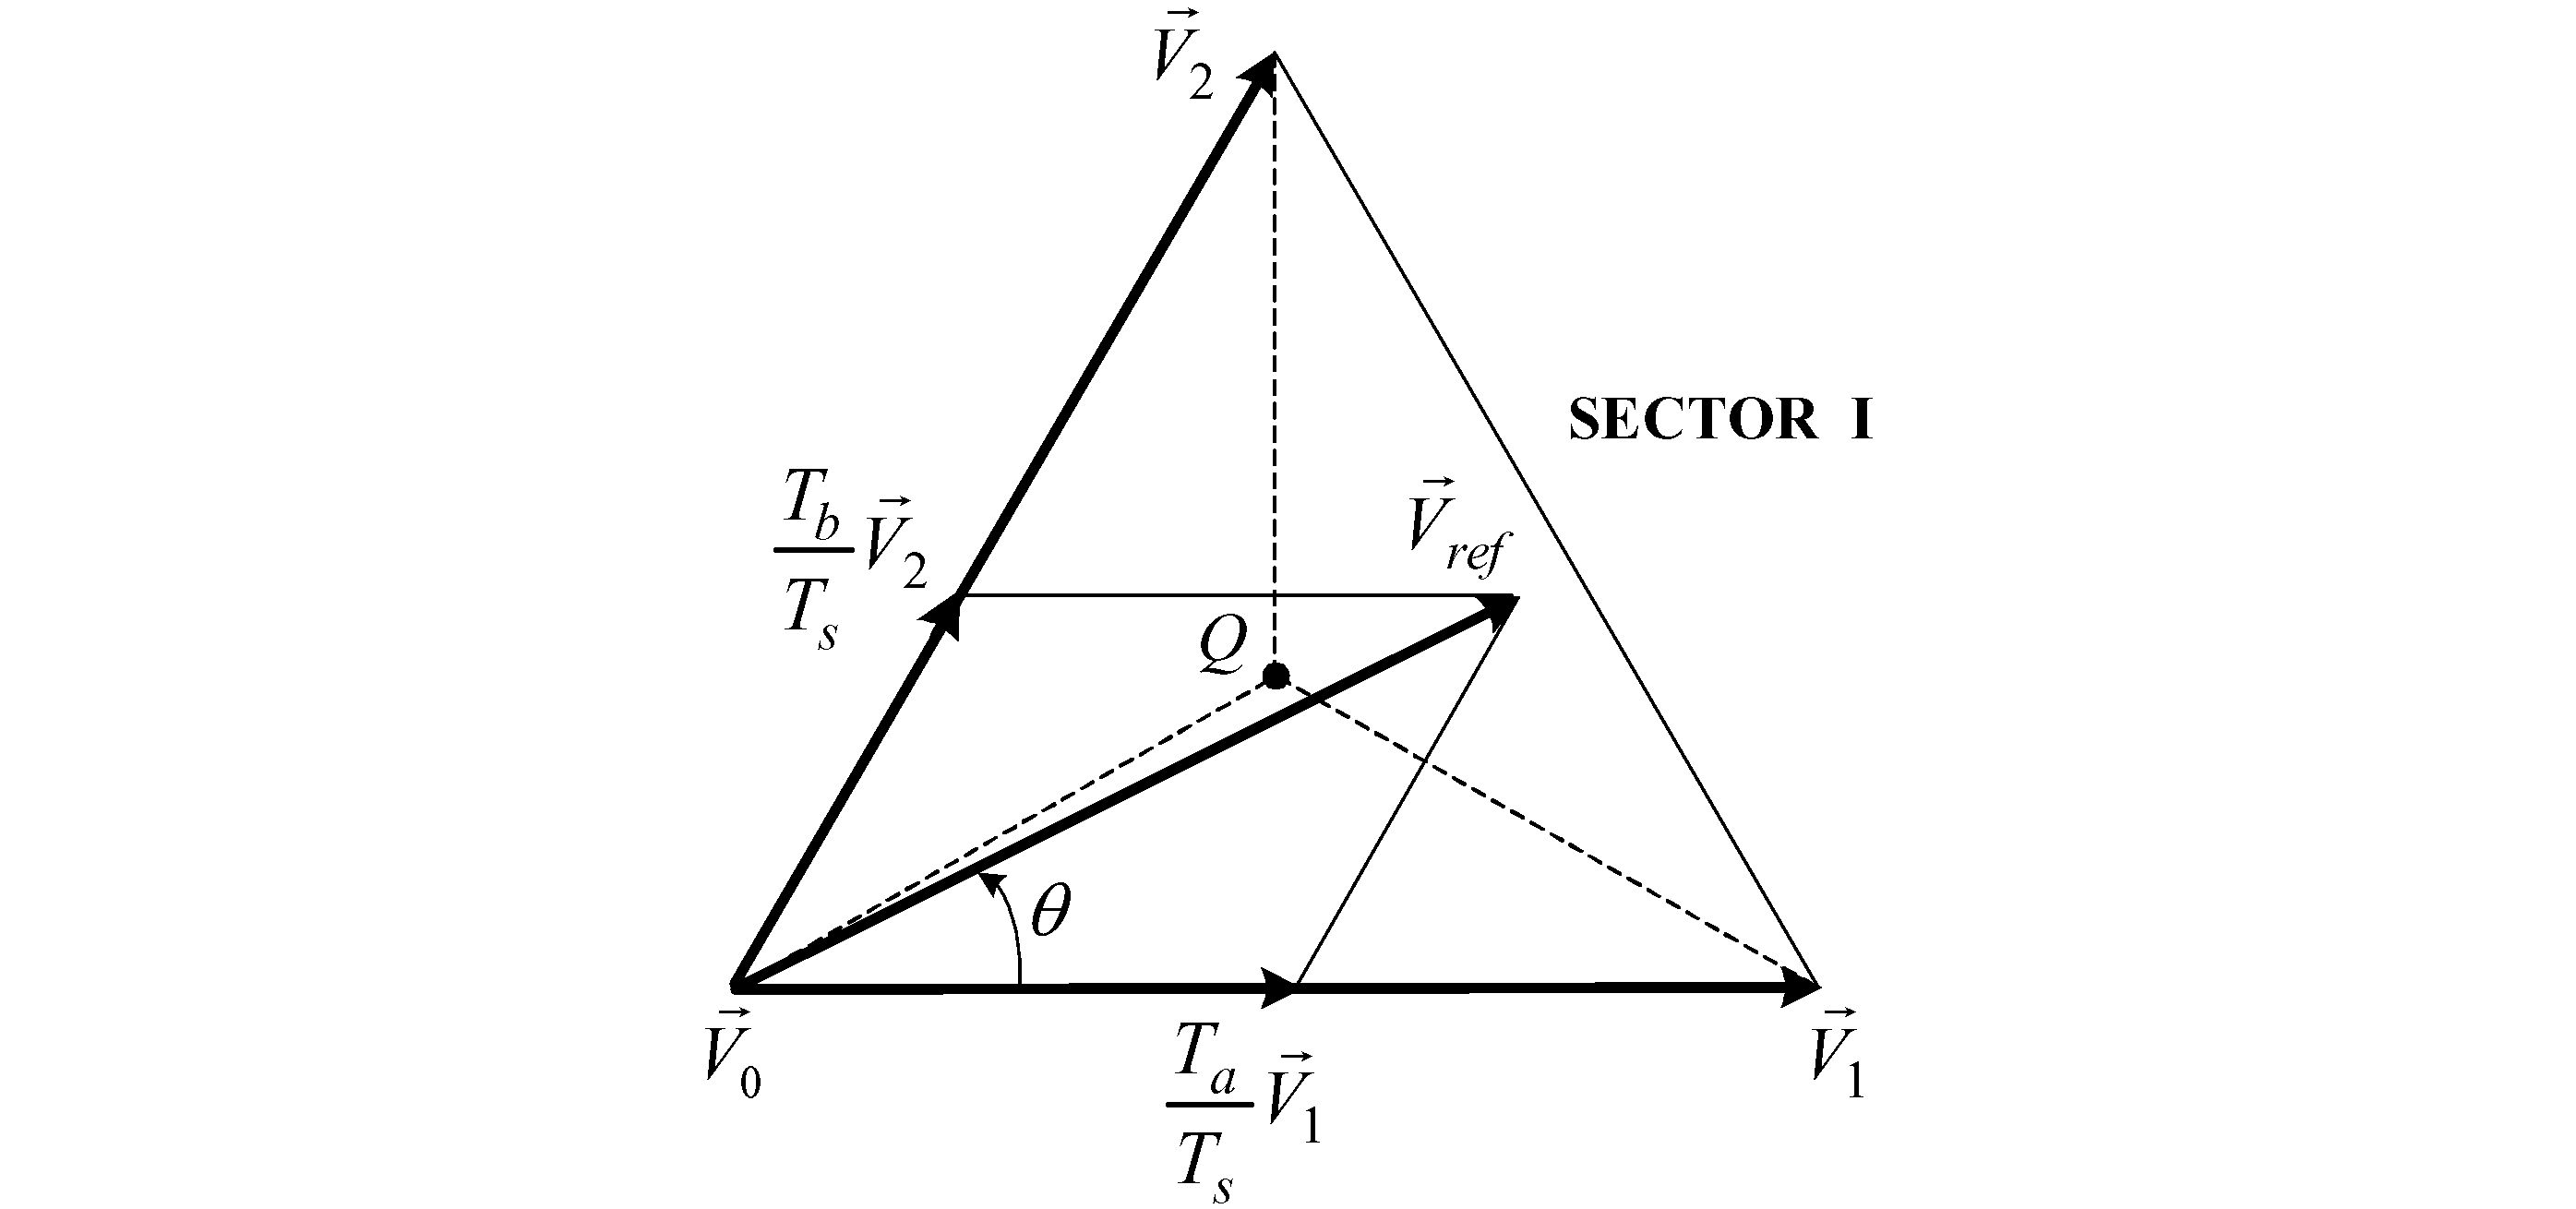
\includegraphics[width=0.8\textwidth]{graficos/img113.jpg}
    \caption{Figura 6.3-2 \( \mathbf{V}_{\text{ref}} \) sintetizado por \( \mathbf{V}_1 \), \( \mathbf{V}_2 \) y \( \mathbf{V}_0 \).}
    \label{fig:sintesis_vectores_espacio}
\end{figure}
\FloatBarrier
    
cae en el sector I como se muestra en la Figura 6.3-2, puede sintetizarse por \( \mathbf{V}_1 \), \( \mathbf{V}_2 \) y \( \mathbf{V}_0 \). La ecuación de balance de volt-segundos es
\[
\mathbf{V}_{\text{ref}} T_s = \mathbf{V}_1 T_a + \mathbf{V}_2 T_b + \mathbf{V}_0 T_0 \tag{6.3-10}
\]
donde \( T_a \), \( T_b \) y \( T_0 \) son los tiempos de dwell para los vectores \( \mathbf{V}_1 \), \( \mathbf{V}_2 \) y \( \mathbf{V}_0 \), respectivamente. Los vectores de espacio en (6.3-10) pueden expresarse como
\[
\mathbf{V}_1 = \frac{2}{3} V_d, \quad \mathbf{V}_2 = \frac{2}{3} V_d e^{j\frac{\pi}{3}}, \quad \text{y} \quad \mathbf{V}_0 = 0 \tag{6.3-11}
\]
    
Sustituyendo (6.3-11) en (6.3-10) y luego separando la ecuación resultante en componentes reales (eje $\alpha$) e imaginarios (eje $\beta$) en el plano $\alpha$-$\beta$, tenemos
\[
\text{Re}: V_{\text{ref}}(\cos \theta) T_s = \frac{2}{3} V_d T_a + \frac{1}{3} V_d T_b \tag{6.3-12}
\]
\[
\text{Im}: V_{\text{ref}}(\sin \theta) T_s = \frac{1}{\sqrt{3}} V_d T_b
\]
    
Resolviendo (6.3-12) junto con \( T_s = T_a + T_b + T_0 \) se obtiene
\[
T_a = \frac{\sqrt{3} V_{\text{ref}}}{V_d} \sin\left(\frac{\pi}{3} - \theta\right), \quad T_b = \frac{\sqrt{3} V_{\text{ref}}}{V_d} \sin \theta \quad \text{para} \quad 0 \leq \theta < \frac{\pi}{3} \tag{6.3-13}
\]
\[
T_0 = T_s - T_a - T_b
\]
    
Para visualizar la relación entre la ubicación de \( \mathbf{V}_{\text{ref}} \) y los tiempos de dwell, examinemos algunos casos especiales. Si \( \mathbf{V}_{\text{ref}} \) se encuentra exactamente en el medio entre \( \mathbf{V}_1 \) y \( \mathbf{V}_2 \) (es decir, \(\theta = \frac{\pi}{6}\)), el tiempo de dwell \( T_a \) para \( \mathbf{V}_1 \) será igual al tiempo de dwell \( T_b \) para \( \mathbf{V}_2 \). Cuando \( \mathbf{V}_{\text{ref}} \) está más cerca de \( \mathbf{V}_1 \) que de \( \mathbf{V}_2 \), \( T_b \) será mayor que \( T_a \). Si \( \mathbf{V}_{\text{ref}} \) coincide con \( \mathbf{V}_2 \), \( T_a \) será cero. Con la cabeza de \( \mathbf{V}_{\text{ref}} \) ubicada justo en el punto central Q en la figura 6.3-2, \( T_a = T_b = T_0 \). La relación entre la ubicación de \( \mathbf{V}_{\text{ref}} \) y los tiempos de dwell se resume en la Tabla 6.3-3.
    
Cabe notar que aunque la Ecuación (6.3-13) se deriva cuando \( \mathbf{V}_{\text{ref}} \) está en el sector I, también puede usarse cuando \( \mathbf{V}_{\text{ref}} \) está en otros sectores siempre que se reste un múltiplo de \( \pi/3 \) del desplazamiento angular real \(\theta\) de modo que el ángulo modificado \(\theta'\) caiga en el rango entre cero y \( \pi/3 \) para su uso en la ecuación, es decir,
\[
\theta' = \theta - (k-1)\frac{\pi}{3} \quad \text{para} \quad 0 \leq \theta' < \frac{\pi}{3} \tag{6.3-14}
\]
donde \( k = 1, 2, \ldots, 6 \) para los sectores I, II, \ldots, VI, respectivamente. Por ejemplo, cuando \( \mathbf{V}_{\text{ref}} \) está en el sector II, los tiempos de dwell calculados \( T_a \), \( T_b \) y \( T_0 \) basados en (6.3-13) y (6.3-14) son para los vectores \( \mathbf{V}_2 \), \( \mathbf{V}_3 \) y \( \mathbf{V}_0 \), respectivamente.

\begin{table}[h]
\centering
\caption{Tabla 6.3-3 Ubicación de \( \mathbf{V}_{\text{ref}} \) y Tiempos de Dwell}
\begin{tabular}{c c c c c c}
\hline
Ubicación de \( \mathbf{V}_{\text{ref}} \) & $\theta = 0$ & $0 < \theta < \frac{\pi}{6}$ & $\theta = \frac{\pi}{6}$ & $\frac{\pi}{6} < \theta < \frac{\pi}{3}$ & $\theta = \frac{\pi}{3}$ \\ [1em]
Tiempos de Dwell: & $T_a > 0$ & $T_a > T_b$ & $T_a = T_b$ & $T_a < T_b$ & $T_a = 0$ \\
& $T_b = 0$ & & & & $T_b > 0$ \\
\hline
\end{tabular}
\end{table}
\FloatBarrier

\subsection*{6.3.4 Índice de Modulación}
    
La Ecuación (6.3-13) también puede expresarse en términos del índice de modulación \( m_a \):
\[
T_a = T_{m_a} \sin\left(\frac{\pi}{3} - \theta\right), \quad T_b = T_{m_a} \sin \theta \quad \text{y} \quad T_0 = T_s - T_a - T_b \tag{6.3-15}
\]
donde
\[
m_a = \frac{\sqrt{3} V_{\text{ref}}}{V_d} \tag{6.3-16}
\]
    
La magnitud máxima del vector de referencia, \( V_{\text{ref},\text{max}} \), corresponde al radio del círculo más grande que puede inscribirse dentro del hexágono mostrado en la Figura 6.3-1. Dado que el hexágono está formado por seis vectores activos que tienen una longitud de \( \frac{2}{3} V_d \), \( V_{\text{ref},\text{max}} \) se puede encontrar a partir de
\[
V_{\text{ref},\text{max}} = \frac{2}{3} V_d \times \frac{\sqrt{3}}{2} = \frac{V_d}{\sqrt{3}} \tag{6.3-17}
\]
    
Sustituyendo (6.3-17) en (6.3-16) se obtiene el índice de modulación máximo:
\[
m_{a,\text{max}} = 1
\]
    
de lo cual el índice de modulación para el esquema SVM está en el rango de
\[
0 \leq m_a \leq 1 \tag{6.3-18}
\]
    
La magnitud máxima del voltaje línea a línea (rms) producido por el esquema SVM puede calcularse por
\[
V_{\text{max},SVM} = \sqrt{3} \left(\frac{V_{\text{ref},\text{max}}}{\sqrt{2}}\right) = 0.707V_d \tag{6.3-19}
\]
    
donde \( \frac{V_{\text{ref},\text{max}}}{\sqrt{2}} \) es el valor rms máximo del voltaje de fase fundamental del inversor.
    
Con el inversor controlado por el esquema SPWM, el voltaje línea a línea fundamental máximo es
\[
V_{\text{max,SPWM}} = 0.612V_d
\]
    
de donde
\[
\frac{V_{\text{max,SVM}}}{V_{\text{max,SPWM}}} = 1.155
\]
    
La Ecuación (6.3-21) indica que para un voltaje de bus DC dado, el voltaje línea a línea máximo generado por el esquema SVM es un 15.5\% mayor que el generado por el esquema SPWM. Sin embargo, el uso del esquema SPWM con inyección de armónico de tercer orden también puede aumentar el voltaje de salida del inversor en un 15.5\%. Por lo tanto, los dos esquemas tienen esencialmente la misma utilización del voltaje de bus DC.

\subsection*{6.3.5 Secuencia de Conmutación}
    
Con los vectores de espacio seleccionados y los tiempos de dwell calculados, el siguiente paso es organizar la secuencia de conmutación. En general, el diseño de la secuencia de conmutación para un \( \mathbf{V}_{\text{ref}} \) dado no es único, pero debe satisfacer los siguientes dos requisitos para minimizar la frecuencia de conmutación de los dispositivos:
    
\begin{enumerate}
    \item La transición de un estado de conmutación a otro involucra solo dos interruptores en la misma rama del inversor, uno siendo encendido y el otro apagado.
    \item La transición para \( \mathbf{V}_{\text{ref}} \) moviéndose de un sector en el diagrama de vectores de espacio al siguiente no requiere ninguna conmutación o requiere un número mínimo de conmutaciones.
\end{enumerate}
    
La Figura 6.3-3 muestra una típica \textit{secuencia de conmutación de siete segmentos} y las formas de onda del voltaje de salida del inversor para \( \mathbf{V}_{\text{ref}} \) en el sector I, donde \( \mathbf{V}_{\text{ref}} \) se sintetiza por \( \mathbf{V}_1 \), \( \mathbf{V}_2 \) y \( \mathbf{V}_0 \). El período de muestreo \( T_s \) se divide en siete segmentos para los vectores seleccionados. Se puede observar lo siguiente:
    
\begin{itemize}
    \item Los tiempos de dwell para los siete segmentos suman el período de muestreo (\( T_s = T_a + T_b + T_0 \)).
    \item Se cumple el requisito de diseño (a). Por ejemplo, la transición de [000] a [POO] se logra encendiendo \( S_1 \) y apagando \( S_4 \), lo que involucra solo dos interruptores.
    \item Los estados de conmutación redundantes para \( \mathbf{V}_0 \) se utilizan para reducir el número de conmutaciones por período de muestreo. Para el segmento de \( T/4 \) en el centro del período de muestreo, se selecciona el estado de conmutación [PPP], mientras que para los segmentos de \( T_d/4 \) a ambos lados, se utiliza el estado [000].
    \item Cada uno de los interruptores en el inversor se enciende y apaga una vez por período de muestreo. La frecuencia de conmutación \( f_{\text{sw}} \) de los dispositivos es igual a la frecuencia de muestreo \( f_{\text{sp}} \), es decir, \( f_{\text{sw}} = f_{\text{sp}} = \frac{1}{T_s} \).
\end{itemize}
    
\begin{figure}[h]
    \centering
    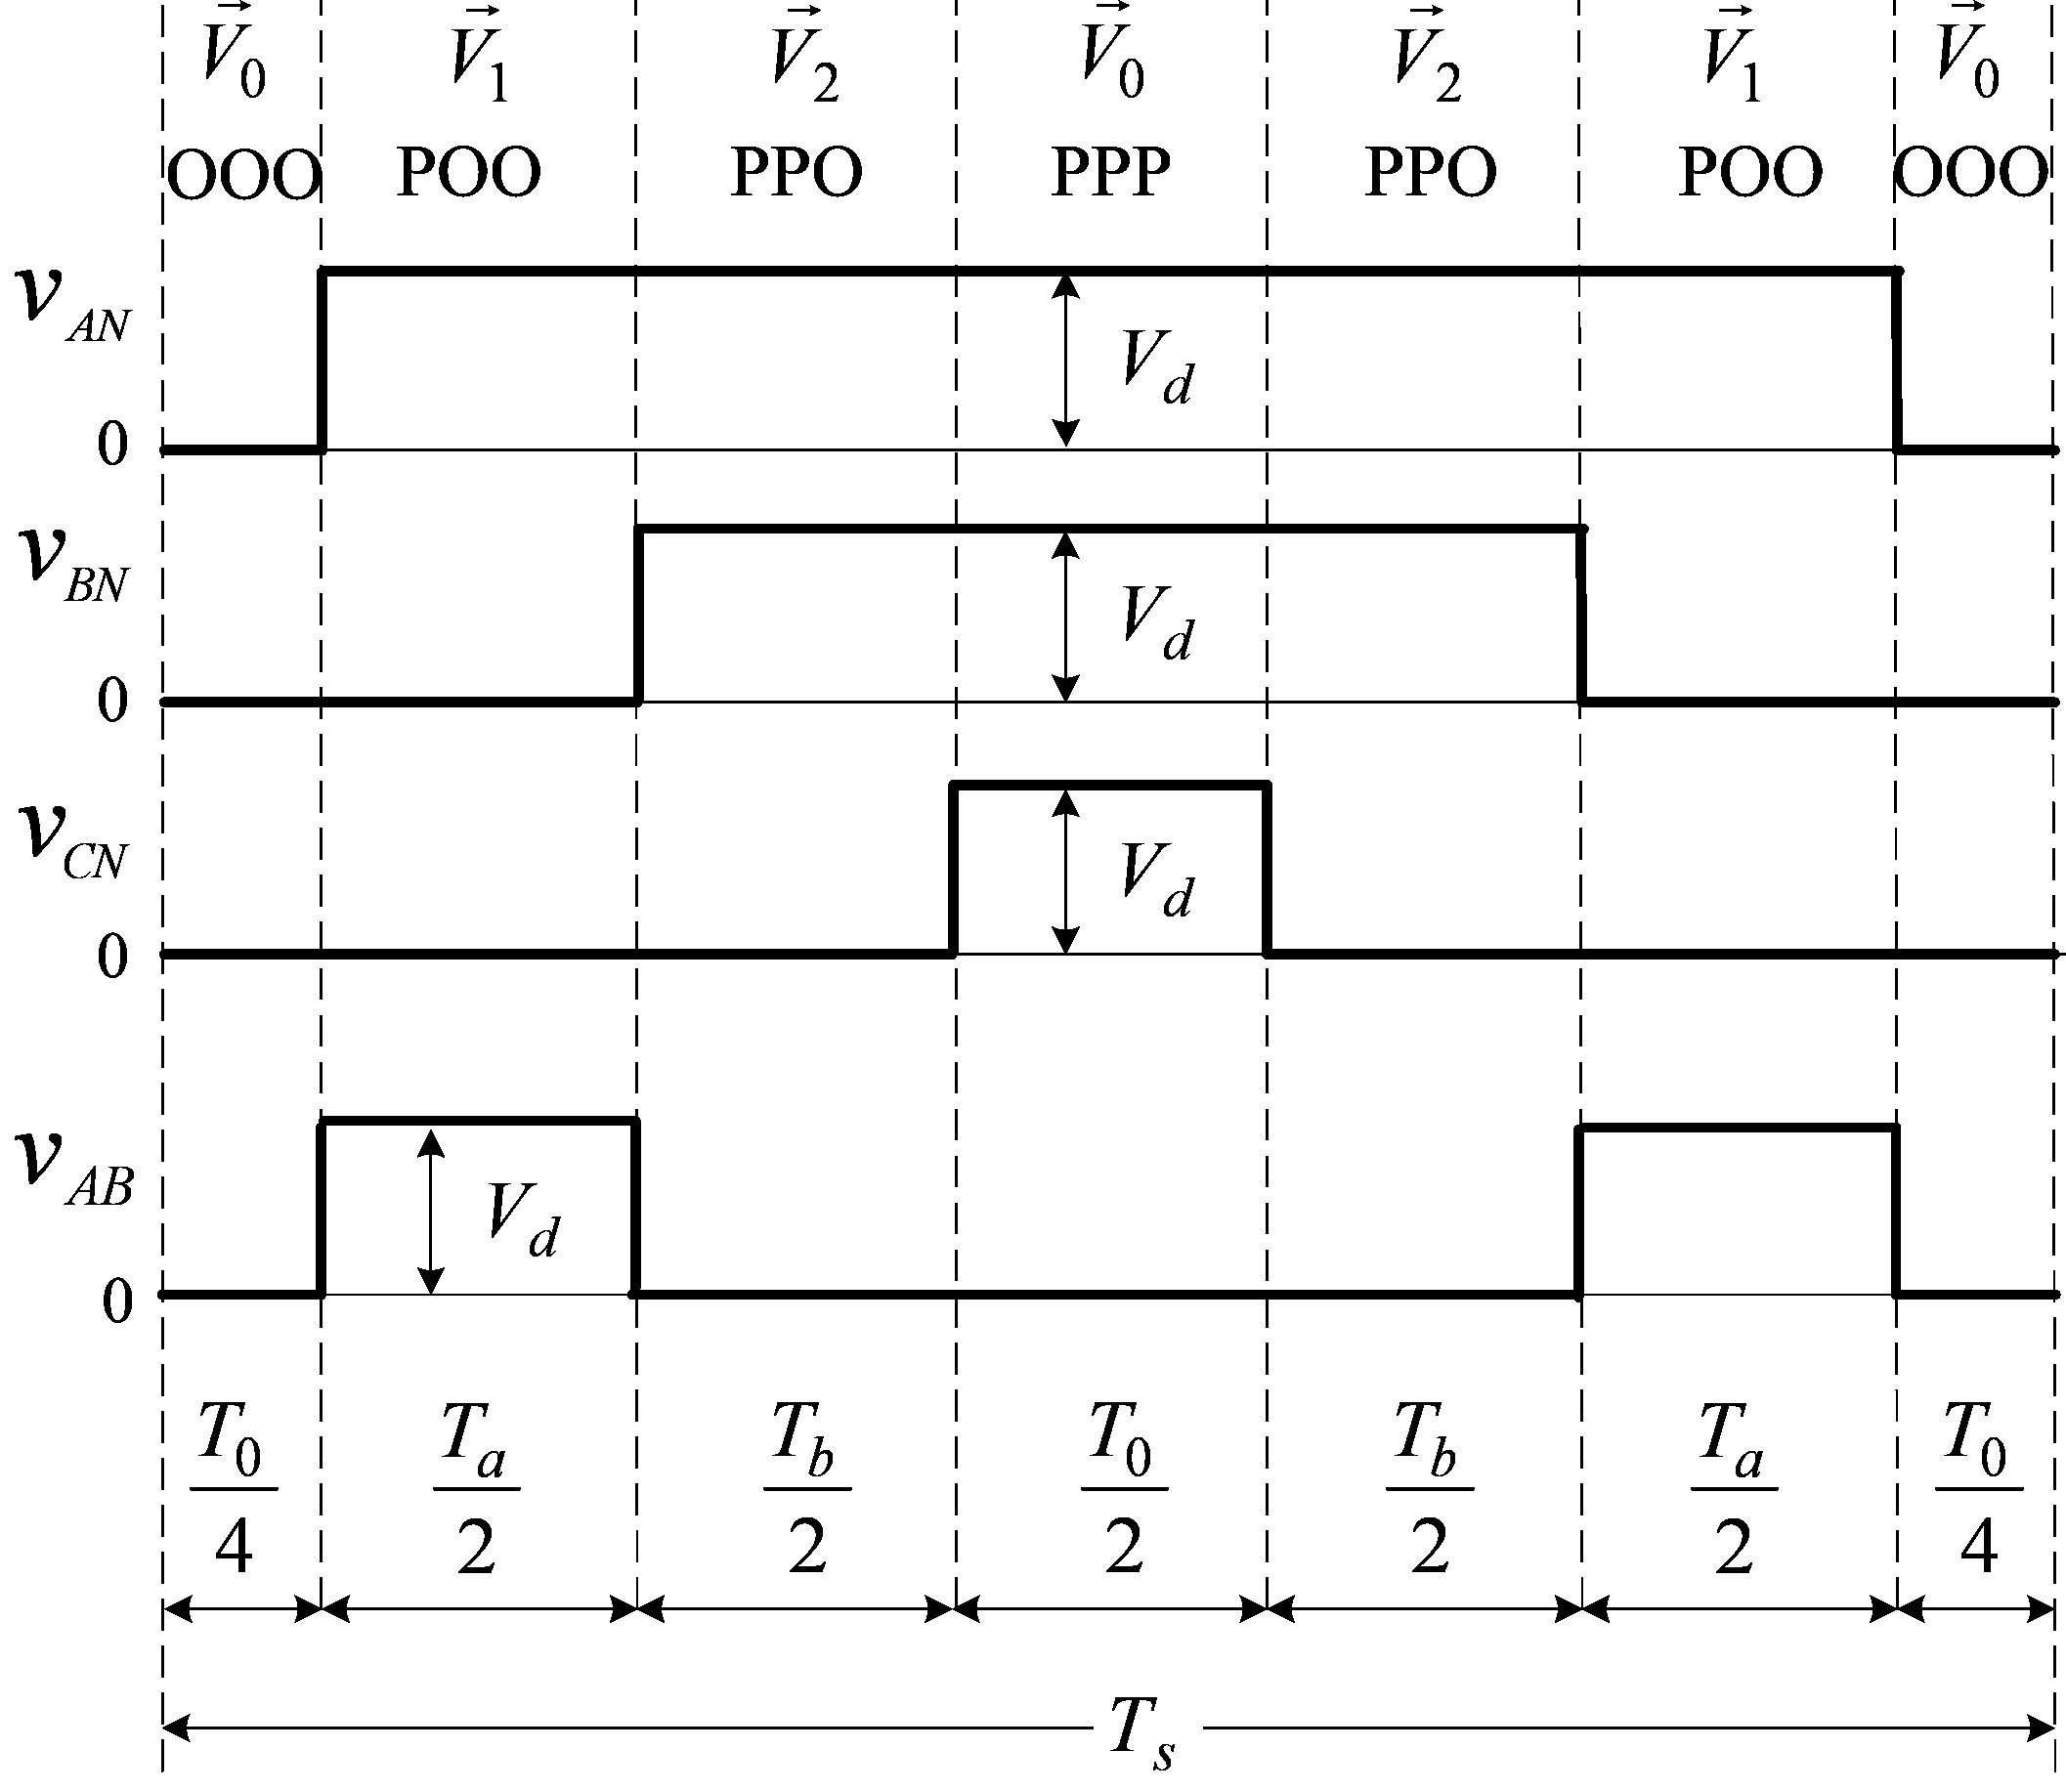
\includegraphics[width=0.8\textwidth]{graficos/img133.jpg}
    \caption{Figura 6.3-3 Secuencia de conmutación de siete segmentos para \( \mathbf{V}_{\text{ref}} \) en el sector I.}
    \label{fig:secuencia_conmutacion_7_segmentos}
\end{figure}
\FloatBarrier
    
Examinemos ahora un caso dado en la Figura 6.3-4, donde los vectores \( \mathbf{V}_1 \) y \( \mathbf{V}_2 \) en la Figura 6.3-3 se intercambian. Algunas transiciones de estados de conmutación, como la transición de [000] a [PPO], se logran encendiendo y apagando cuatro interruptores en dos ramas del inversor simultáneamente. Como consecuencia, el número total de conmutaciones durante el período de muestreo aumenta de seis en el caso anterior a diez. Obviamente, esta secuencia de conmutación no cumple con el requisito de diseño y, por lo tanto, no debe adoptarse.
    
Es interesante notar que las formas de onda de \( V_{AB} \) en las Figuras 6.3-3 y 6.3-4 producidas por dos secuencias de conmutación diferentes parecen diferentes, pero son esencialmente las mismas. Si estas dos formas de onda se dibujan para dos o más períodos de muestreo consecutivos, notaremos que son idénticas excepto por un pequeño retraso de tiempo (\( T/2 \)). Dado que \( T_s \) es mucho más corto que el período de la frecuencia fundamental del inversor, el efecto causado por el retraso de tiempo es negligente.
    
La Tabla 6.3-4 da las secuencias de conmutación de siete segmentos para \( \mathbf{V}_{\text{ref}} \) residiendo en los seis sectores. Note que todas las secuencias de conmutación comienzan y terminan con el estado de conmutación [000], lo que indica que la transición para \( \mathbf{V}_{\text{ref}} \) moviéndose de un sector al siguiente no requiere ninguna conmutación. Se cumple el requisito de diseño (b).

\begin{table}[h]
\centering
\caption{Tabla 6.3-4 Secuencias de Conmutación de Siete Segmentos para Todos los Sectores}
\begin{tabular}{c c c c c c c}
\hline
Sector & 1 & 2 & 3 & 4 & 5 & 6 \\
\hline
Secuencia de Conmutación & [000] [POO] [V1] [V2] [PPP] [V2] [V1] [000] & [000] [PPO] [V2] [V3] [PPP] [V3] [V2] [000] & [000] [OPO] [V3] [V4] [PPP] [V4] [V3] [000] & [000] [OPP] [V4] [V5] [PPP] [V5] [V4] [000] & [000] [OOP] [V5] [V6] [PPP] [V6] [V5] [000] & [000] [POP] [V6] [V1] [PPP] [V1] [V6] [000] \\
\hline
\end{tabular}
\end{table}
\FloatBarrier

\subsection*{6.3.6 Análisis Espectral}
    
Las formas de onda simuladas para los voltajes de salida del inversor y la corriente de carga se muestran en la Figura 6.3-5. El inversor opera bajo la condición de \( f_1 = 60 \text{ Hz} \), \( T_s = 1/720 \text{ s} \), \( f_{\text{sw}} = 720 \text{ Hz} \), y \( m_a = 0.8 \) con una carga inductiva trifásica nominal. El factor de potencia de la carga es 0.9 por fase. Se puede observar que la forma de onda del voltaje de salida del inversor y la corriente de carga son sinusoidales con mínima distorsión armónica.

\begin{figure}[h]
    \centering
    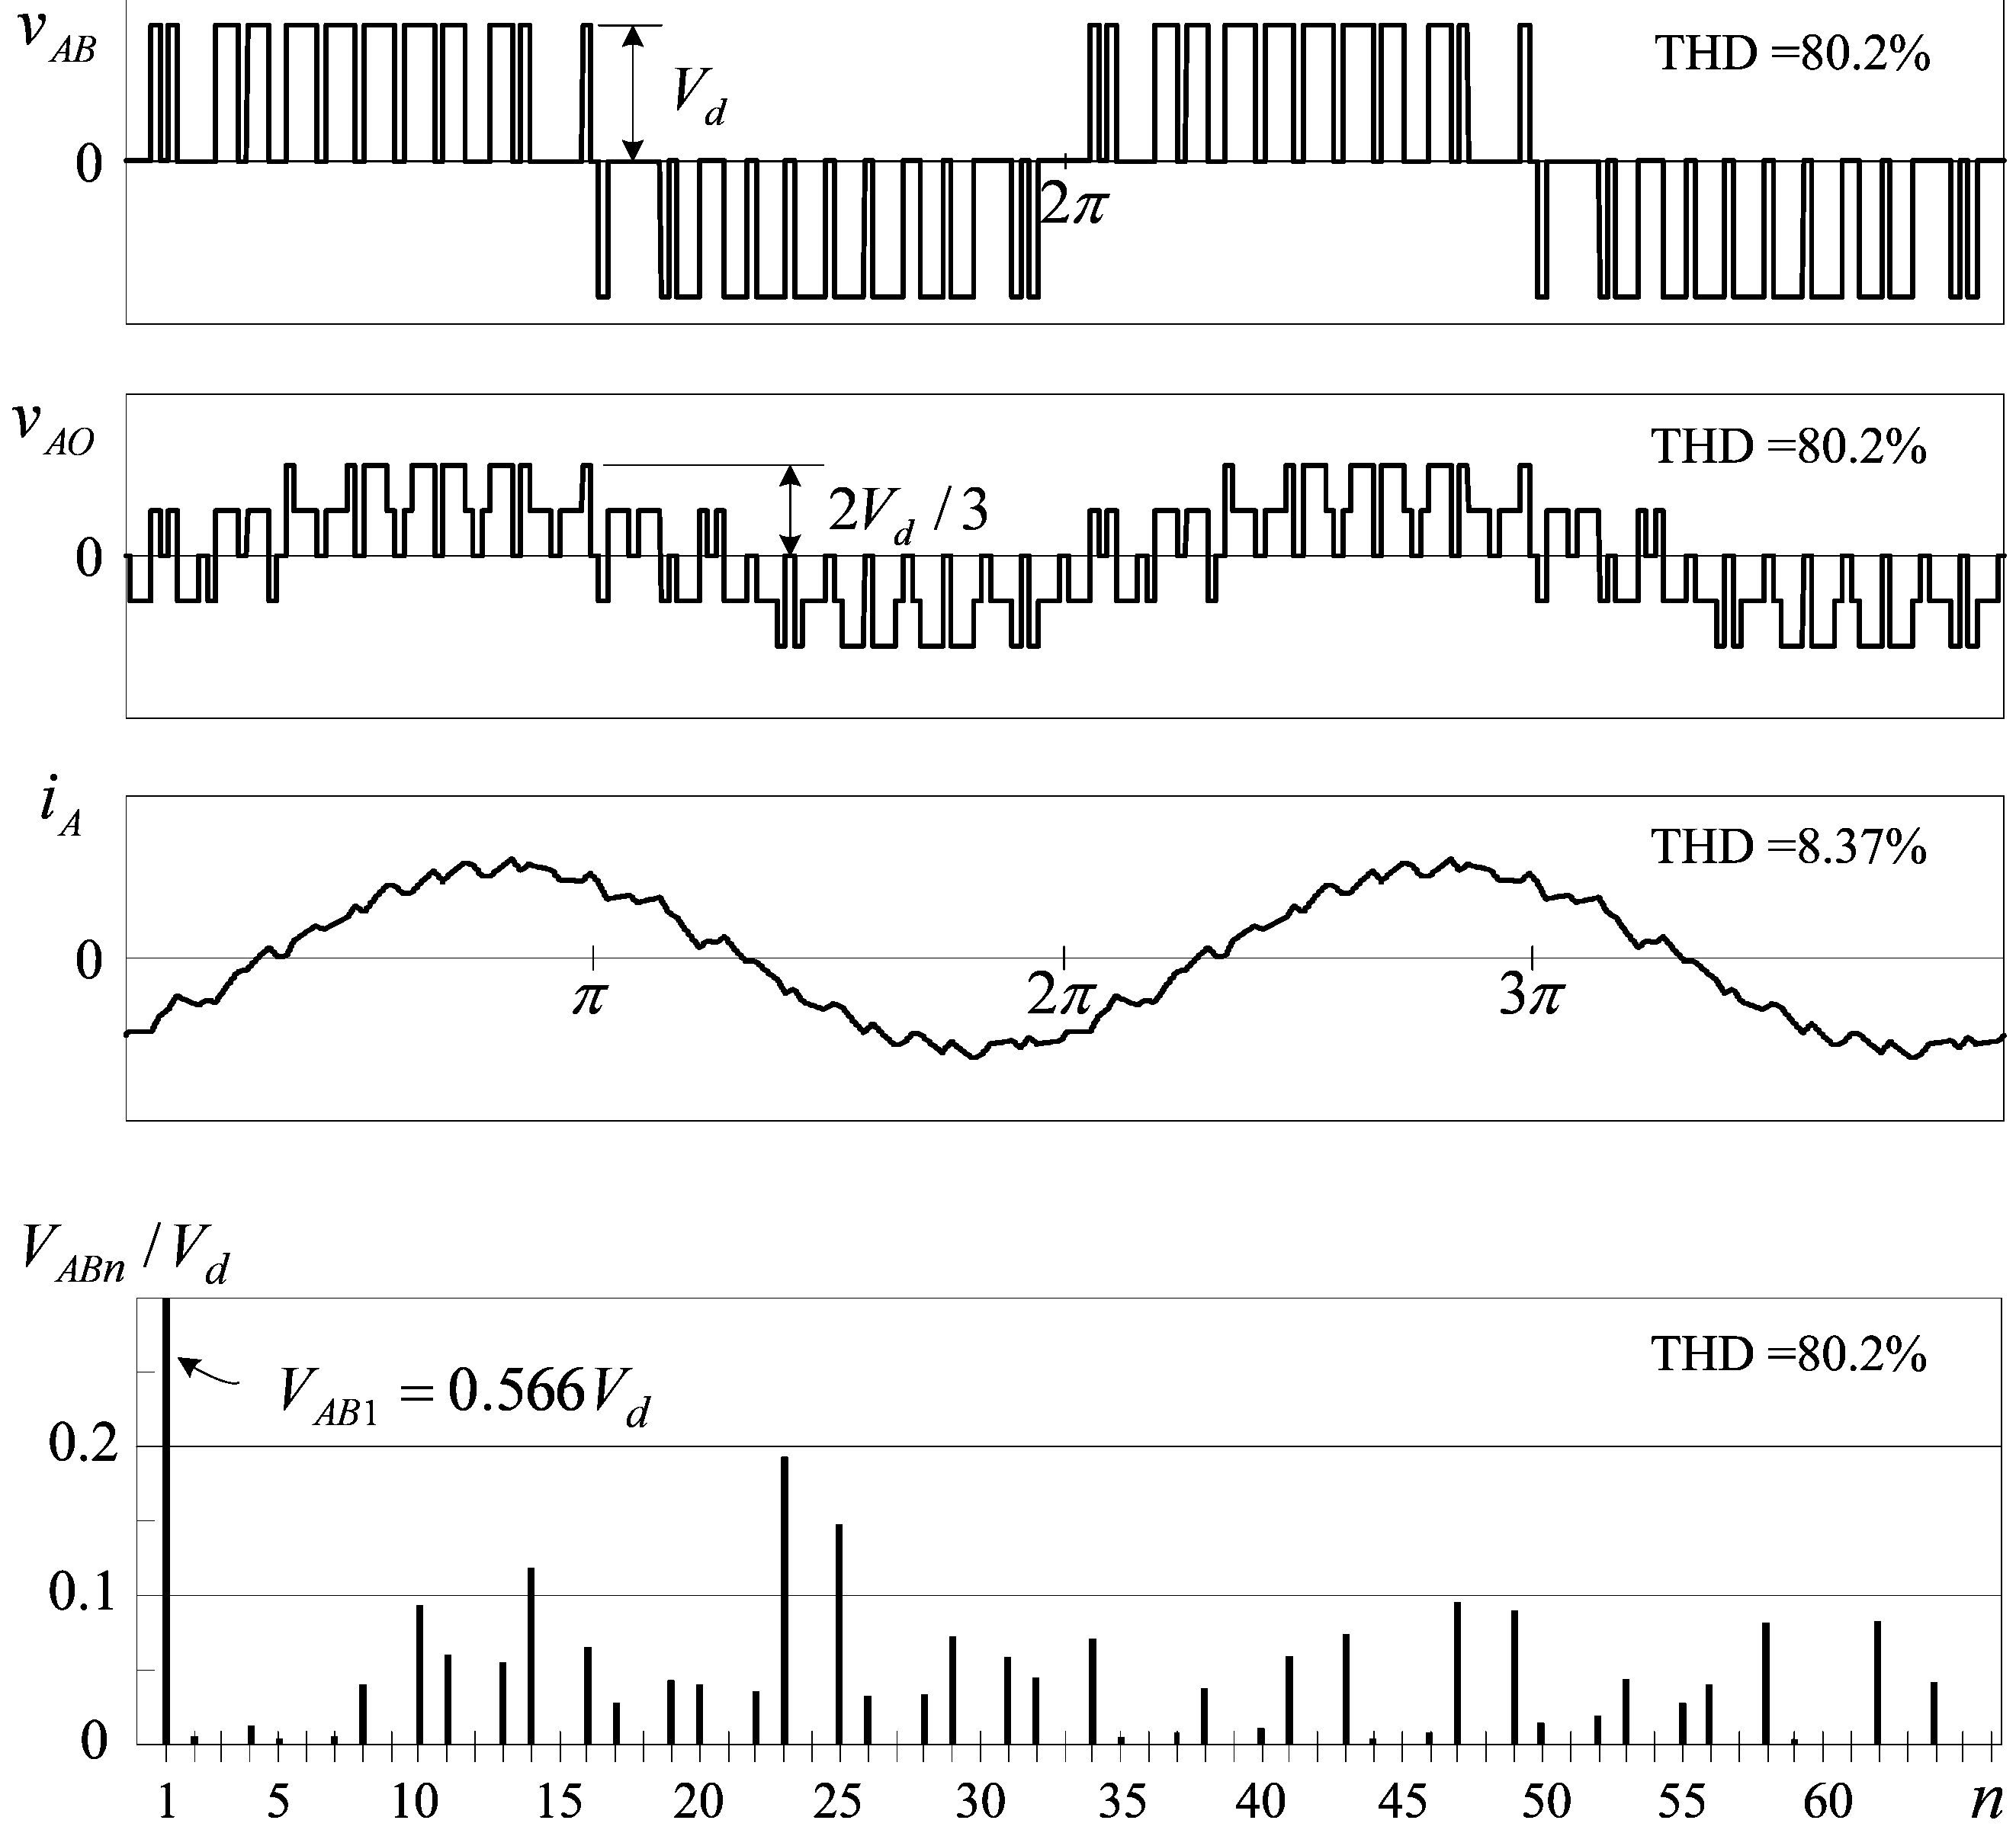
\includegraphics[width=0.8\textwidth]{graficos/img143.jpg}
    \caption{Figura 6.3-5 Formas de onda simuladas del voltaje de salida del inversor y la corriente de carga.}
    \label{fig:analisis_espectral}
\end{figure}
\FloatBarrier

\bibliographystyle{plain}
\bibliography{referencias}

\end{document}
